%%%%%%%%%%%%%%%%%%%%%%%%%%%%%%%%%%%%%%%%%%%%%%%%%%%%%%%%%%%
%%%%%%%%%%%%%%%%%%%%%%%%%%%%%%%%%%%%%%%%%%%%%%%%%%%%%%%%%%%
\section{Parameter Identification and the MUD Point}
%%%%%%%%%%%%%%%%%%%%%%%%%%%%%%%%%%%%%%%%%%%%%%%%%%%%%%%%%%%
%%%%%%%%%%%%%%%%%%%%%%%%%%%%%%%%%%%%%%%%%%%%%%%%%%%%%%%%%%%

%%%%%%%%%%%%%%%%%%%%%%%%%%%%%%%%%%%%%%%%%%%%%%%%%%%%%%%%%%%
\begin{frame}[t]
\centering
\vskip 24pt
We formally define the maximal updated density (MUD) point as
\begin{equation}\label{eq:mudpt_inital_defn}
	\mudpt := \argmax {\updated}(\param).
\end{equation}

\vskip 24pt
We motivate the use of the MUD point as an alternative to the MAP point for parameter estimation problems.

\end{frame}

\begin{frame}[t]

Let $\norm{\mathbf{x}}_C^2 := (\mathbf{x}, \mathbf{x})_C = \mathbf{x}^T C \mathbf{x}$. \\

Inverse covariances associated with non-degenerative multivariate Gaussian distributions will play the role of $C$. \\

Suppose that the initial and prior densities are both given by the same $\mathcal{N}(\param_0, \initialCov)$ distribution.

\vskip 12pt
Additionally, suppose the map $Q$ is linear and that the data-likelihood and observed densities are both given by the same $\mathcal{N}(\observedMean, \observedCov)$ distribution.

\vskip 12pt
The linearity of $Q$ implies that $Q(\param)=A\param$ for some $A\in\RR^{d\times p}$, and that the predicted density follows a $\mathcal{N}(Q(\param_0), \predictedCov)$ distribution where
\begin{equation}\label{eq:predictCov}
	\predictedCov := A\initialCov A^\top.
\end{equation}

\end{frame}

%%%%%%%%%%%%%%%%%%%%%%%%%%%%%%%%%%%%%%%%%%%%%%%%%%%%%%%%%%
\subsection{Theory of Regularization}
%%%%%%%%%%%%%%%%%%%%%%%%%%%%%%%%%%%%%%%%%%%%%%%%%%%%%%%%%%

\begin{frame}[t]{\it The one with the regularization equations.}
%\vskip 25pt
\centering
\begin{figure}
\centering

\begin{table}[htbp]
\centering

\begin{tabular}{|c|c|}
\hline
  & \\
  $\displaystyle \updated(\param) = \initial(\param) \frac{\observed(Q(\param))}{\predicted(Q(\param))}$
&
  $\displaystyle \pi_{\text{post}}(\param\,|\,d) = \frac{\pi_{\text{prior}}(\param)\pi_\text{like}(d\,|\,\param)}{\int_{\Lambda} \pi_\text{like}(d\, |\, \param)  \pi_{\text{prior}}(\param) d\pmeas}$
\\
\hline
  & \\
  Tikhonov & $T(\param):=\norm{Q(\param)-\observedMean}_{\observedCov^{-1}}^2 +
      \norm{\param-\initialMean}_{\initialCov^{-1}}^2$
  \\ & \\ \hline & \\
  Data-Consistent & $J(\param):=T(\param) - \norm{Q(\param)-Q(\initialMean)}_{\predictedCov^{-1}}^2$
\\
& \\
  \hline
\end{tabular}
\caption{The $\param$ which minimizes these functionals also maximizes the updated PDF (left) and the Bayesian posterior PDF (right).

$T(\param)$ is the typical functional often associated with Tikhonov regularization.

The $J(\param)$ has an additional term subtracted from $T(\param)$ coming from the predicted density that serves as ``unregularization'' in data--informed directions.}
  \label{tab:func_comparisons}
\end{table}


\end{figure}

\end{frame}



%%%%%%%%%%%%%%%%%%%%%%%%%%%%%%%%%%%%%%%%%%%%%%%%%%%%%%%%%%%
\subsection{Linear Example}
%%%%%%%%%%%%%%%%%%%%%%%%%%%%%%%%%%%%%%%%%%%%%%%%%%%%%%%%%%%

%%%%%%%%%%%%%%%%%%%%%%%%%%%%%%%%%%%%%%%%%%%%%%%%%%%%%%%%%%%
\begin{frame}[t]{\it The one where an example highlights a key difference.}

\centering
Consider a linear QoI map is defined by $A=\mat{cc}{1 & 1}$. \\
2-D input, 1-D output $\implies$ rank-deficient

\vskip 12pt

Parameters in the initial and observed densities are given by
\begin{equation*}
\begin{split}
	\initialMean = \mat{cc}{0.25 & 0.25}^\top, \\
  \initialCov = \mat{cc}{1 & -0.25 \\ -0.25 & 0.5}, \\
  \observedMean=1, \text{ and } \observedCov = \mat{c}{0.25}
\end{split}
\end{equation*}

\end{frame}

%%%%%%%%%%%%%%%%%%%%%%%%%%%%%%%%%%%%%%%%%%%%%%%%%%%%%%%%%%%
\begin{frame}[t]
%\vskip 25pt
\centering
\begin{figure}
\centering

\begin{figure}
   % 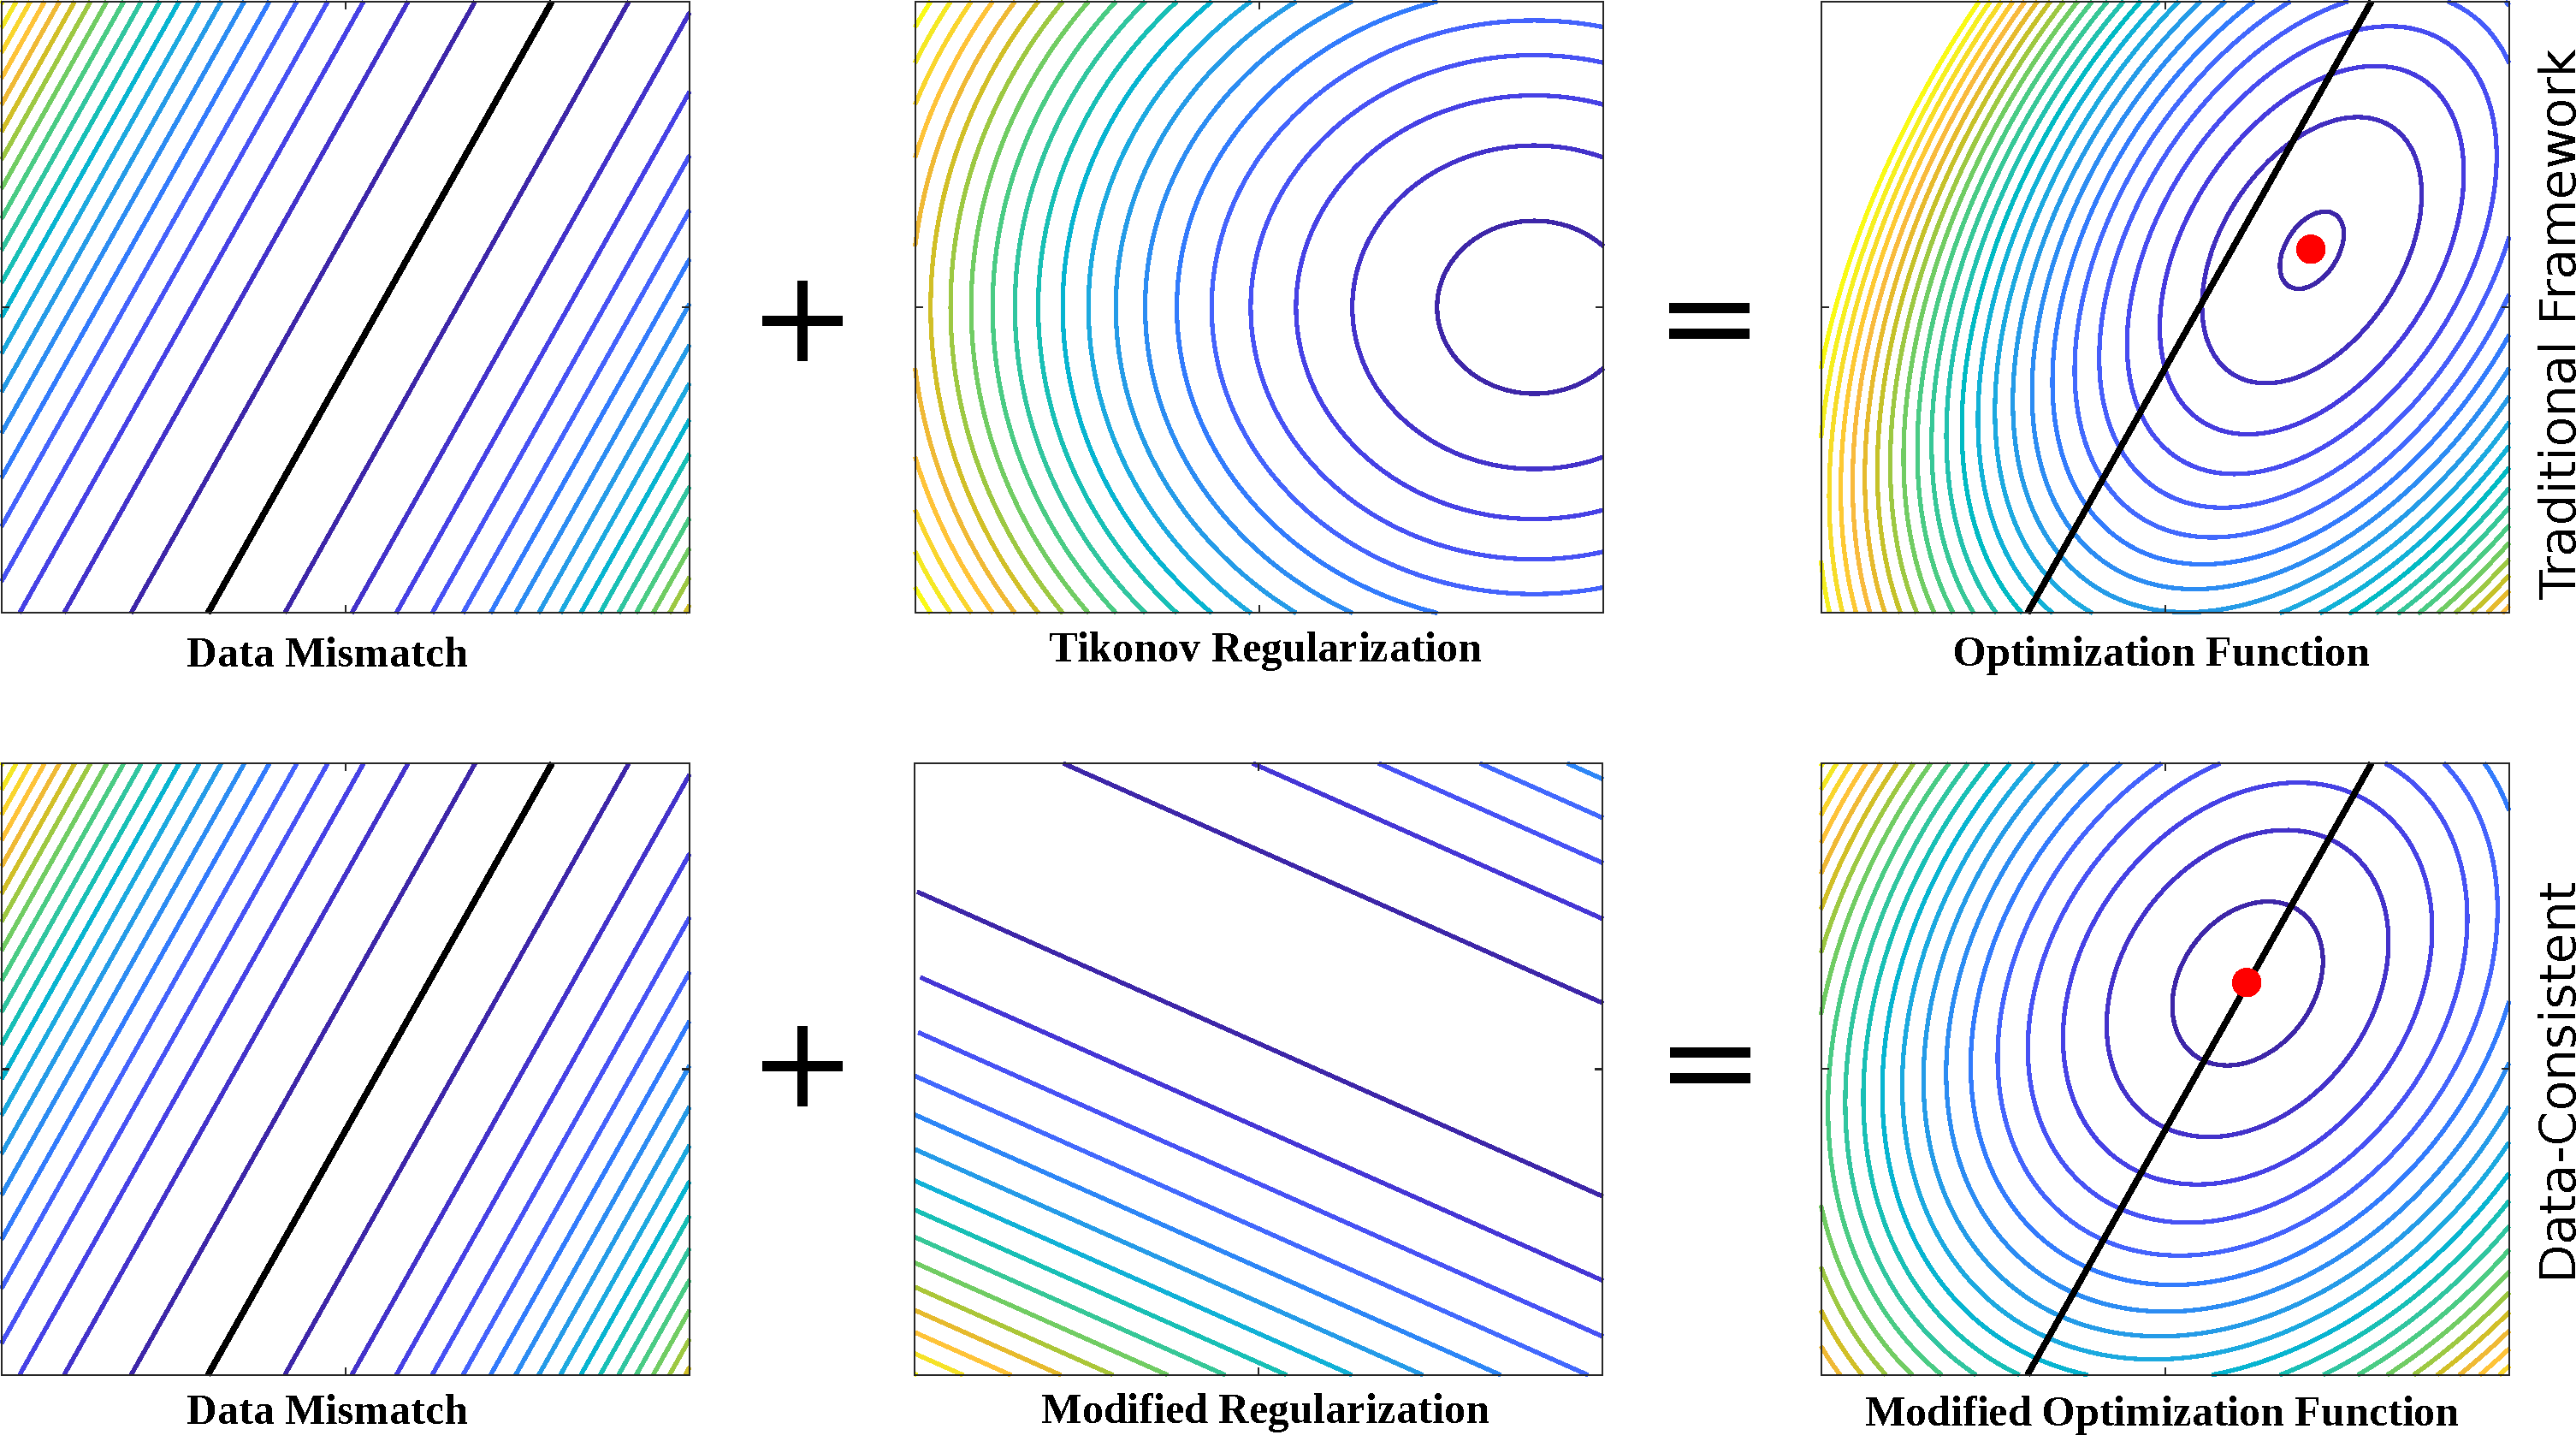
\includegraphics[width=\linewidth]{figures/Regularization-all-in-one.pdf}
  \centering
  \begin{tabular}{|ccc|}
    \hline
      \subf{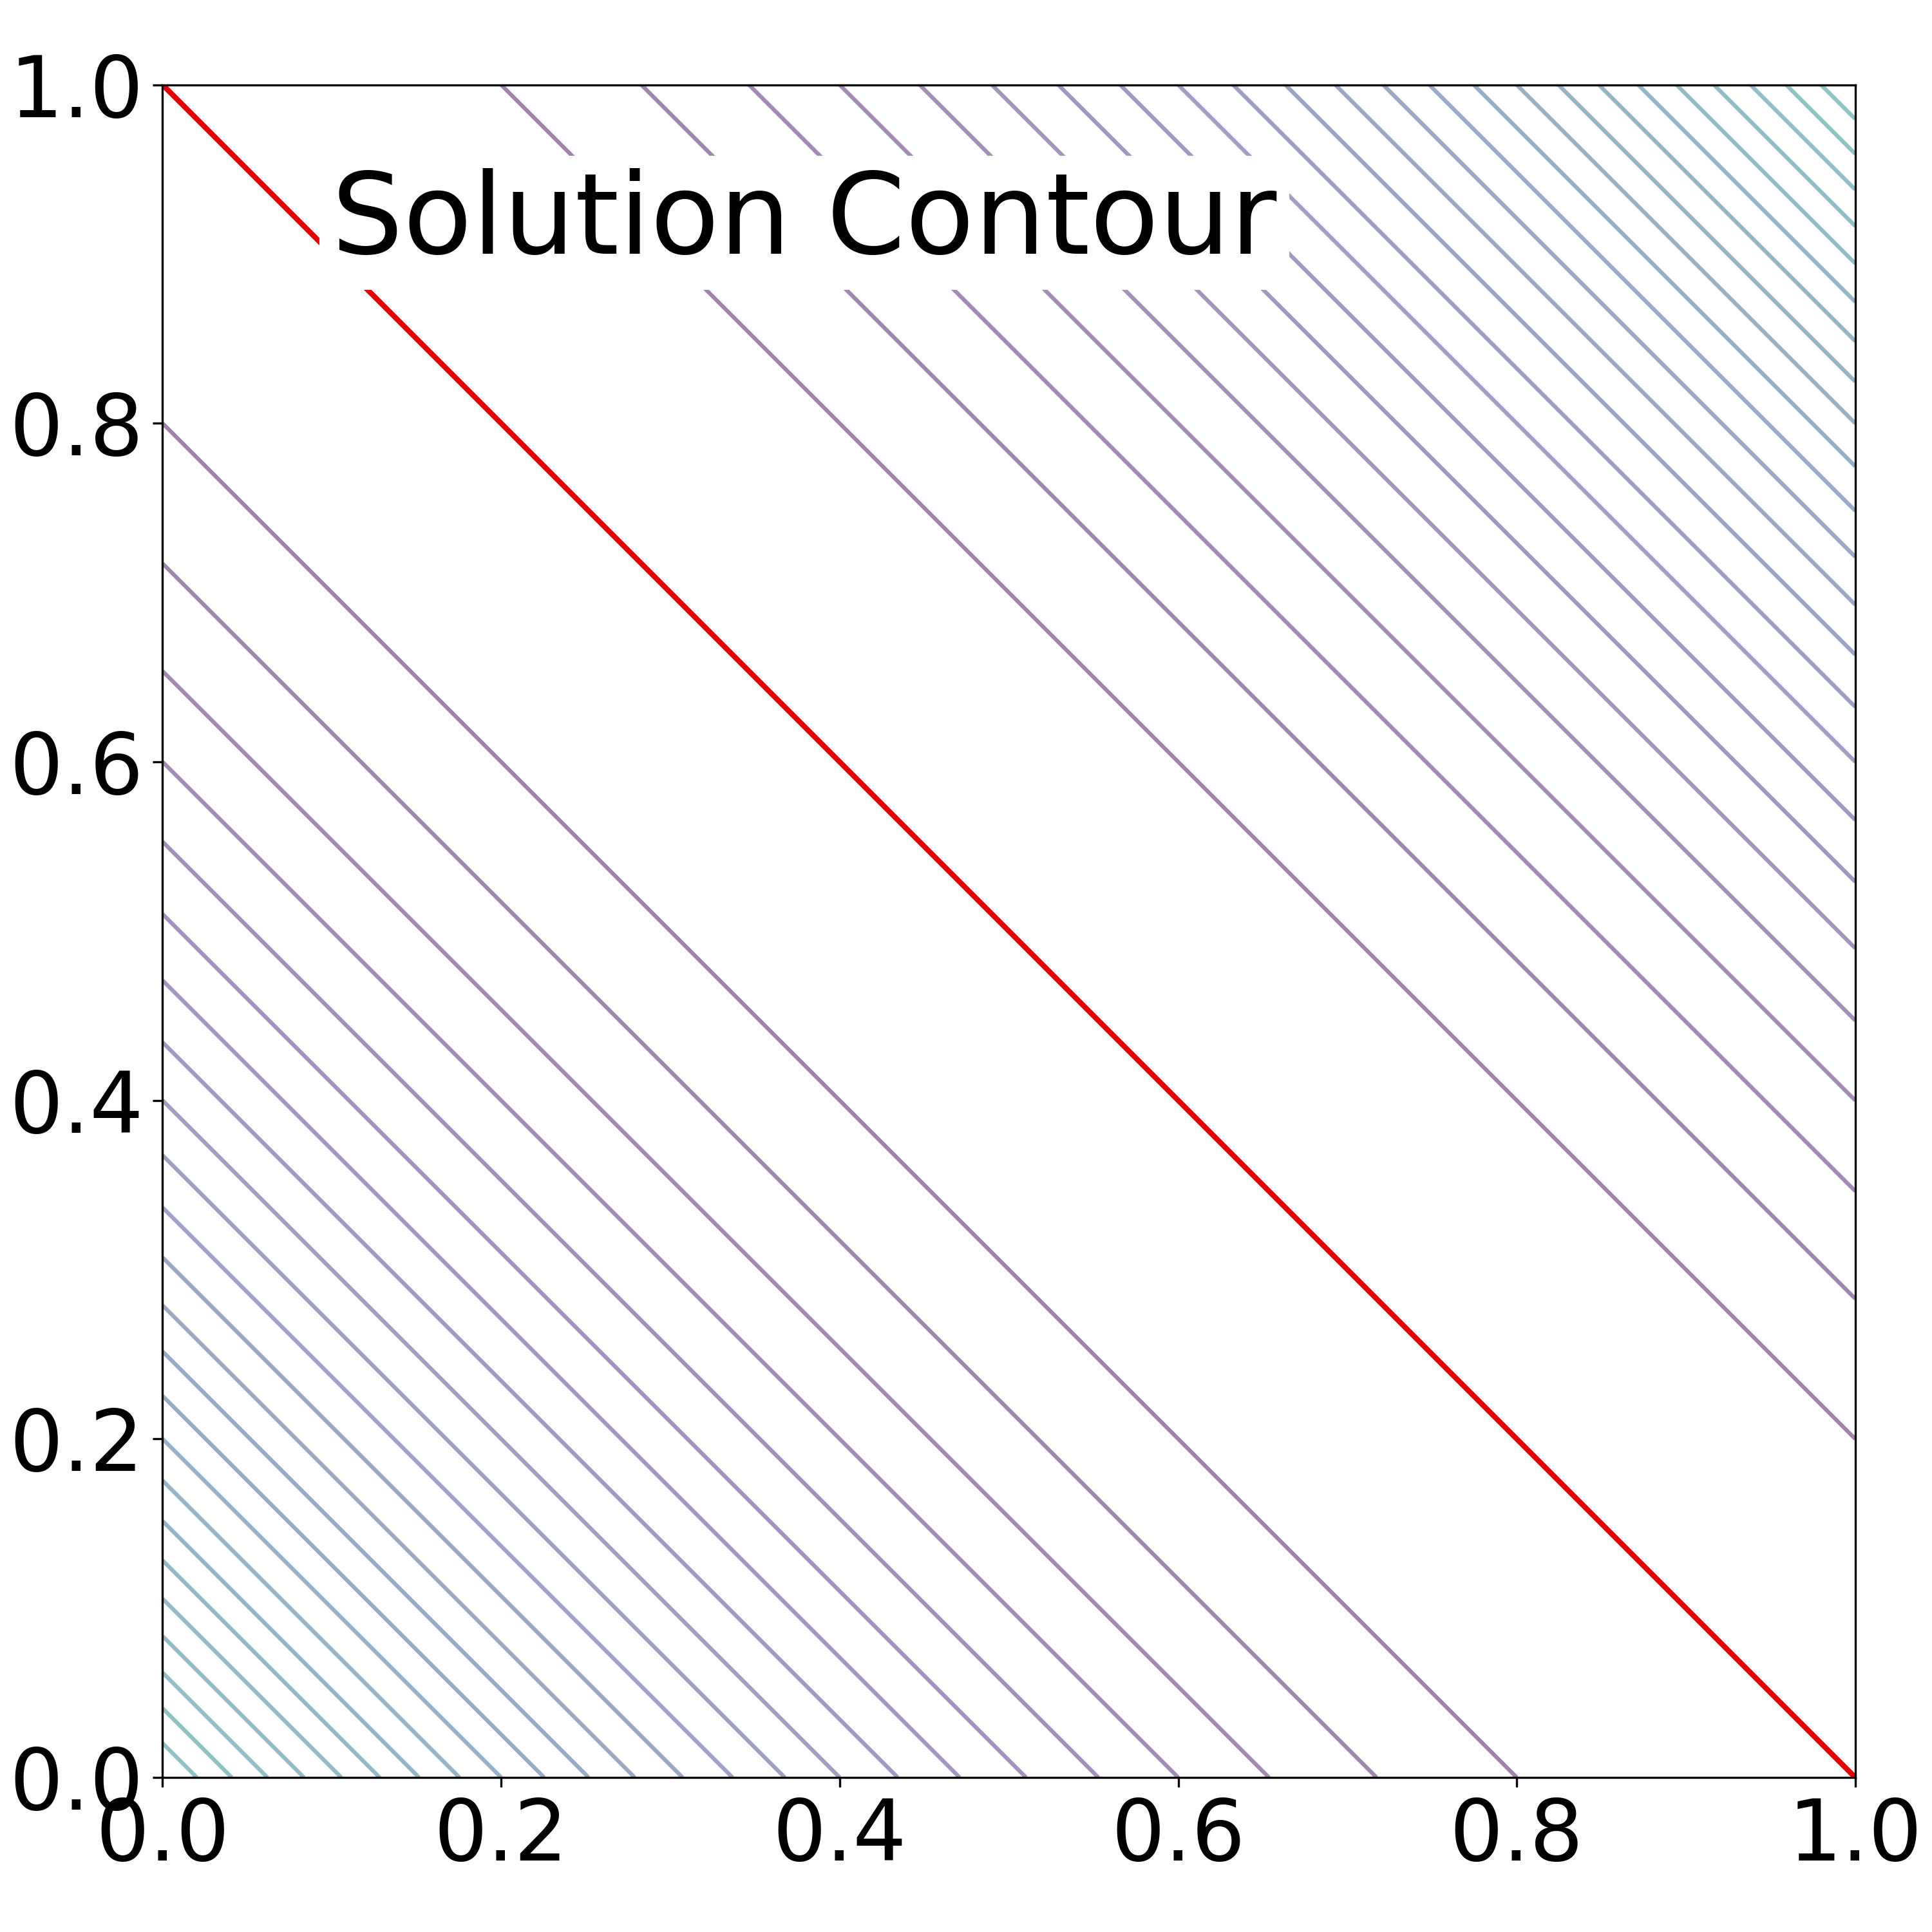
\includegraphics[width=0.25\linewidth]{figures/data_mismatch_contour.png}}
      {data mismatch}
    &
      \subf{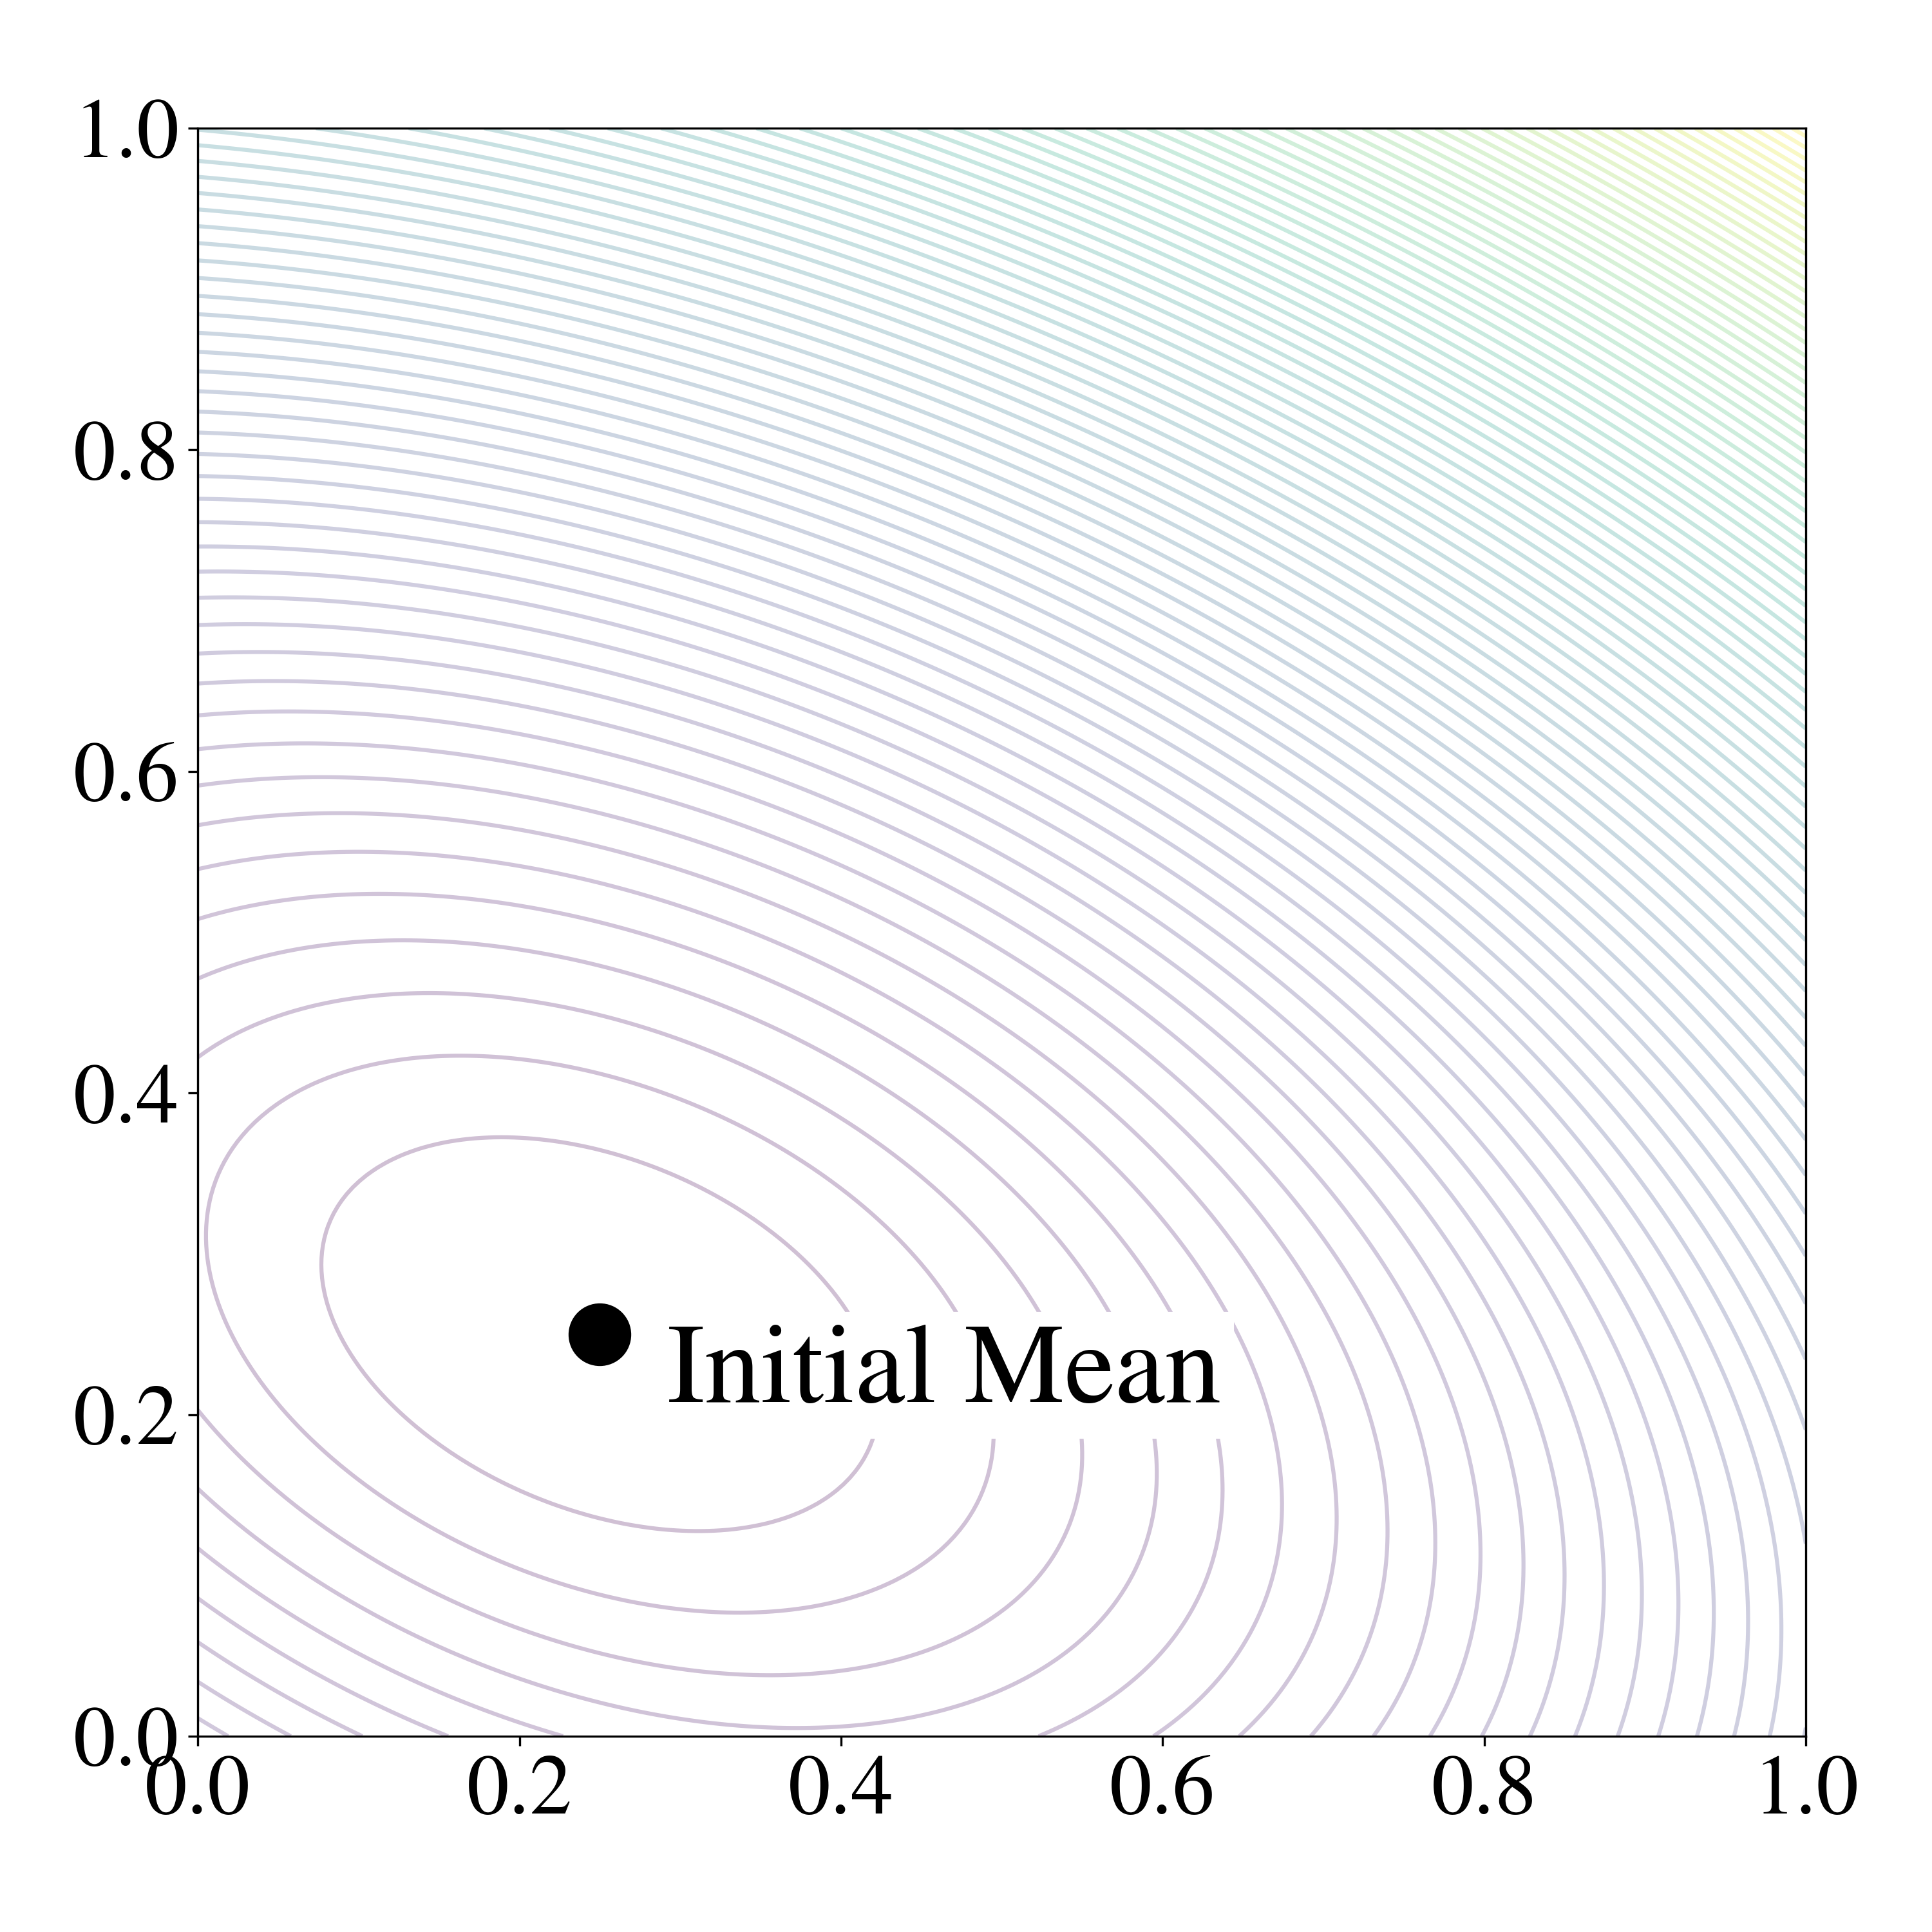
\includegraphics[width=0.25\linewidth]{figures/tikonov_contour.png}}
      {regularization}
    &
      \subf{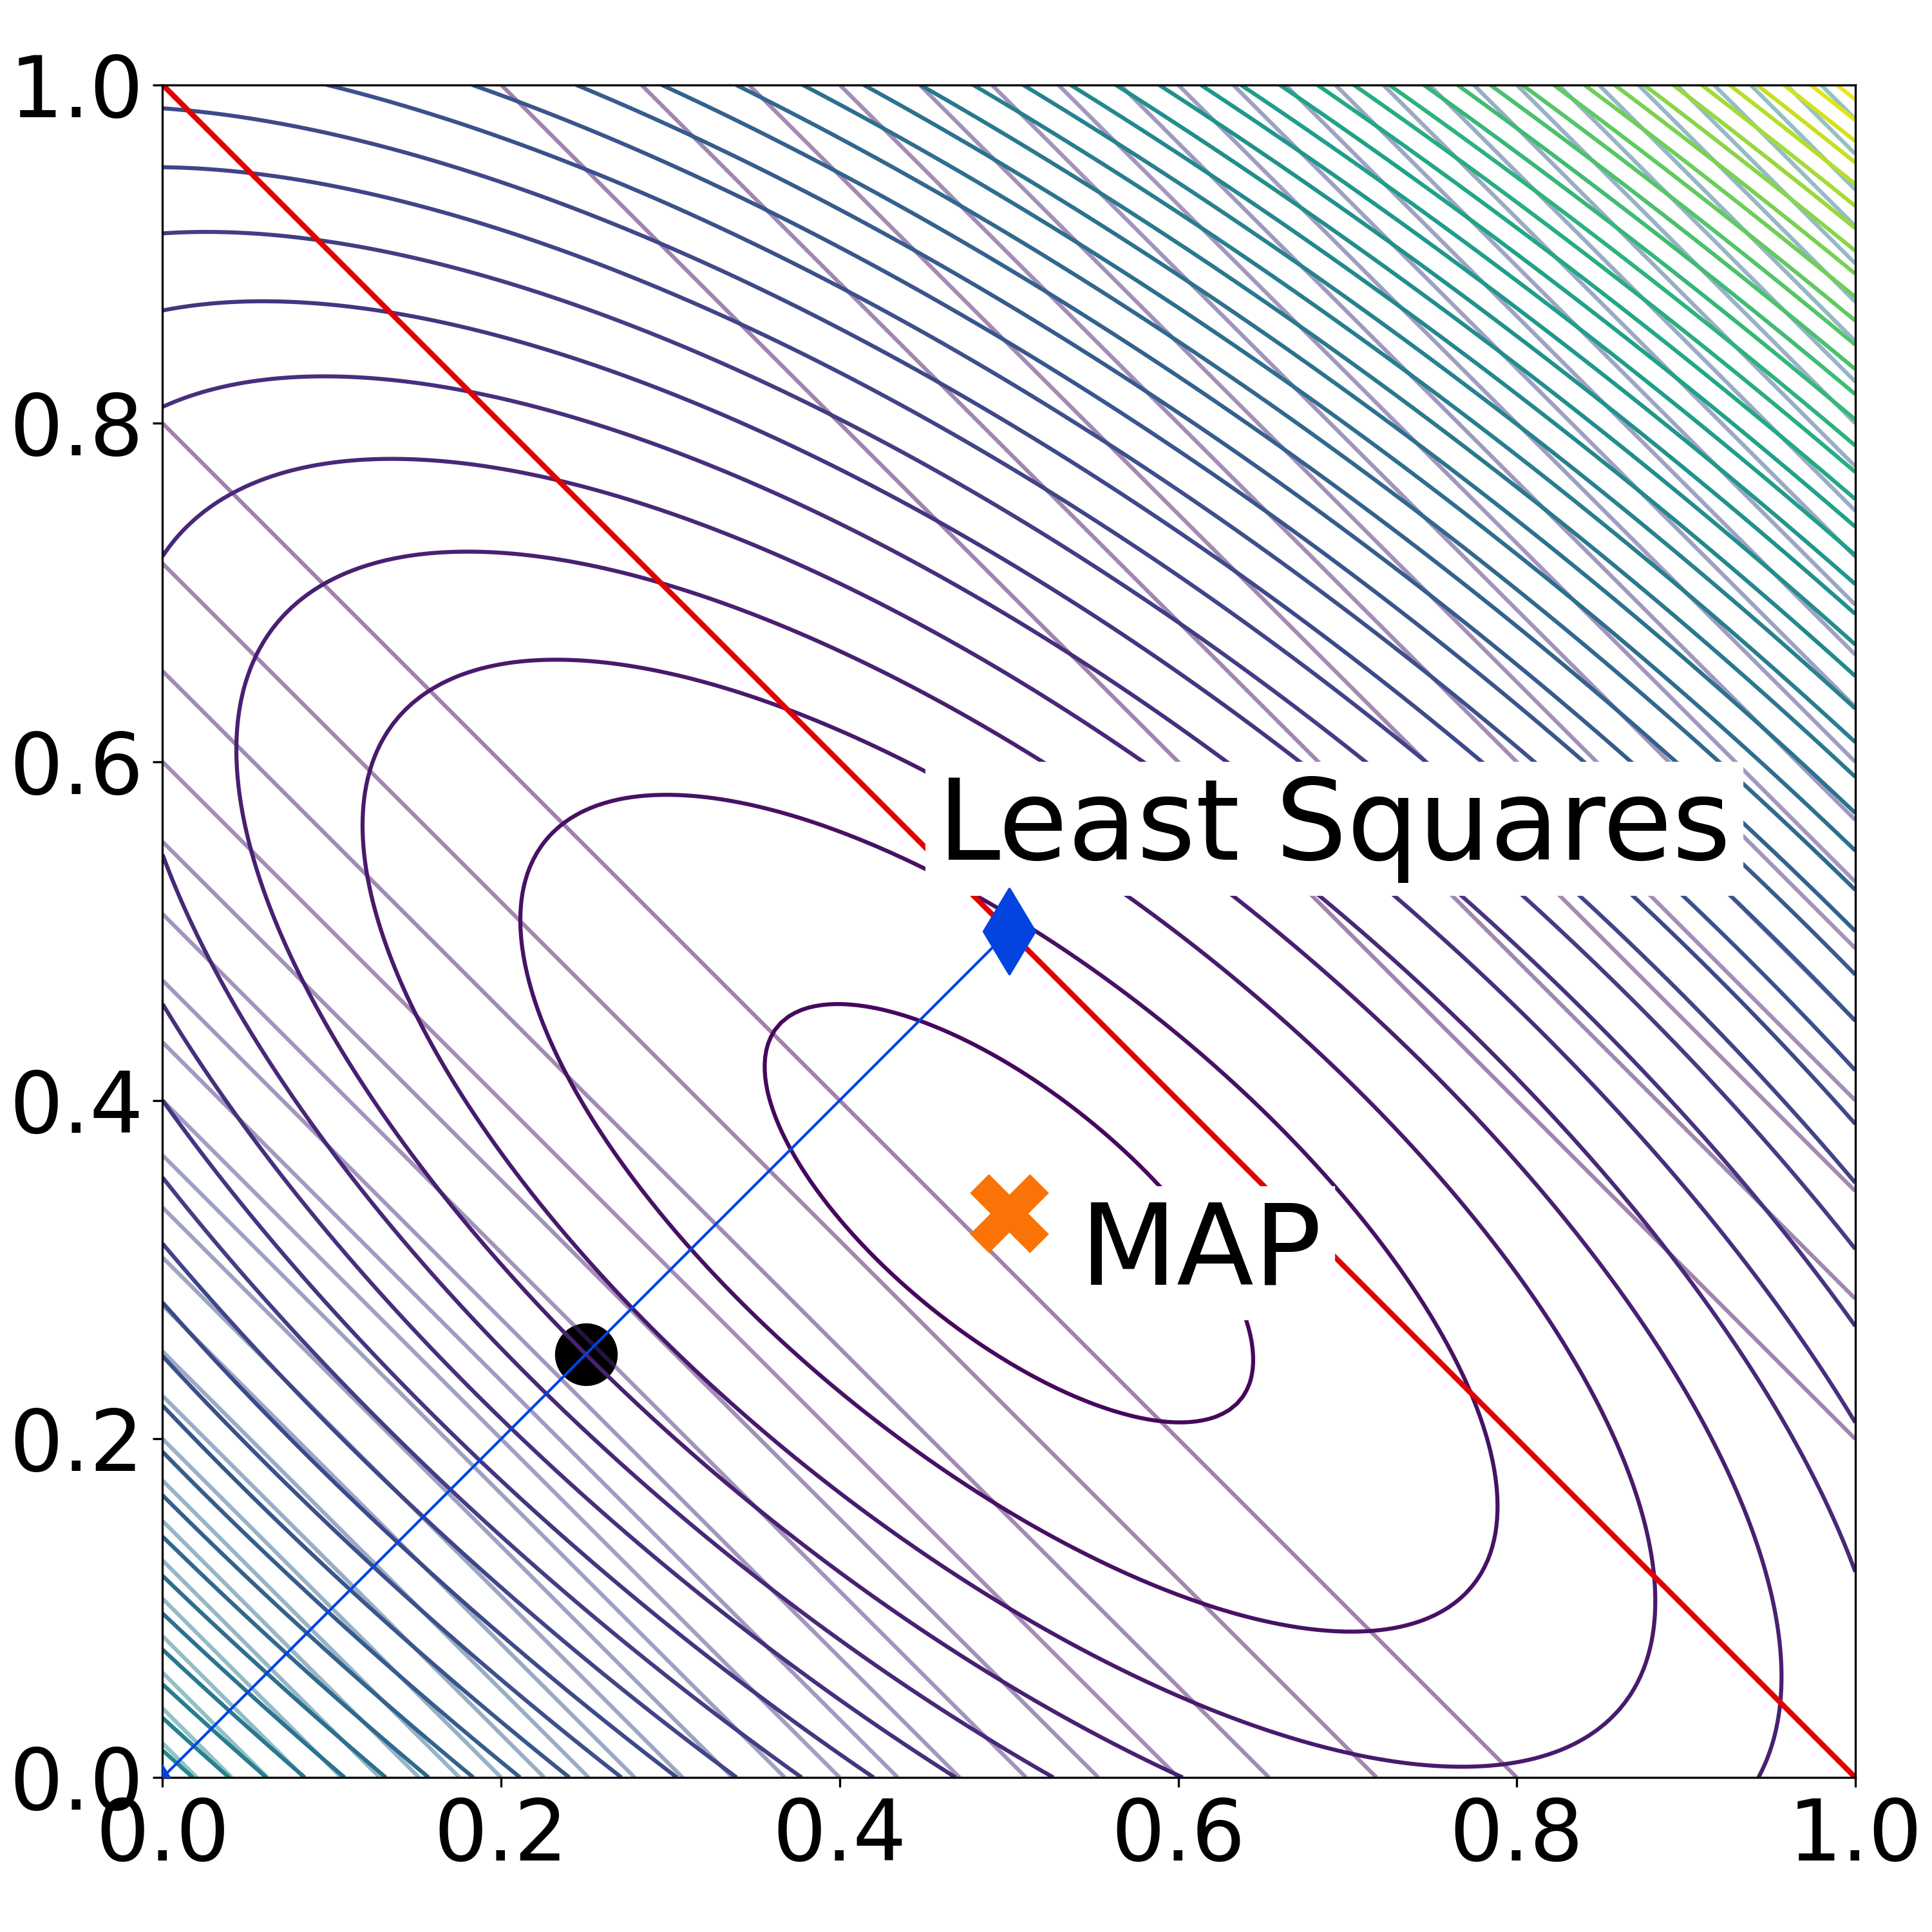
\includegraphics[width=0.25\linewidth]{figures/classical_solution.png}}
      {bayesian posterior}
    \\
    \hline
      \subf{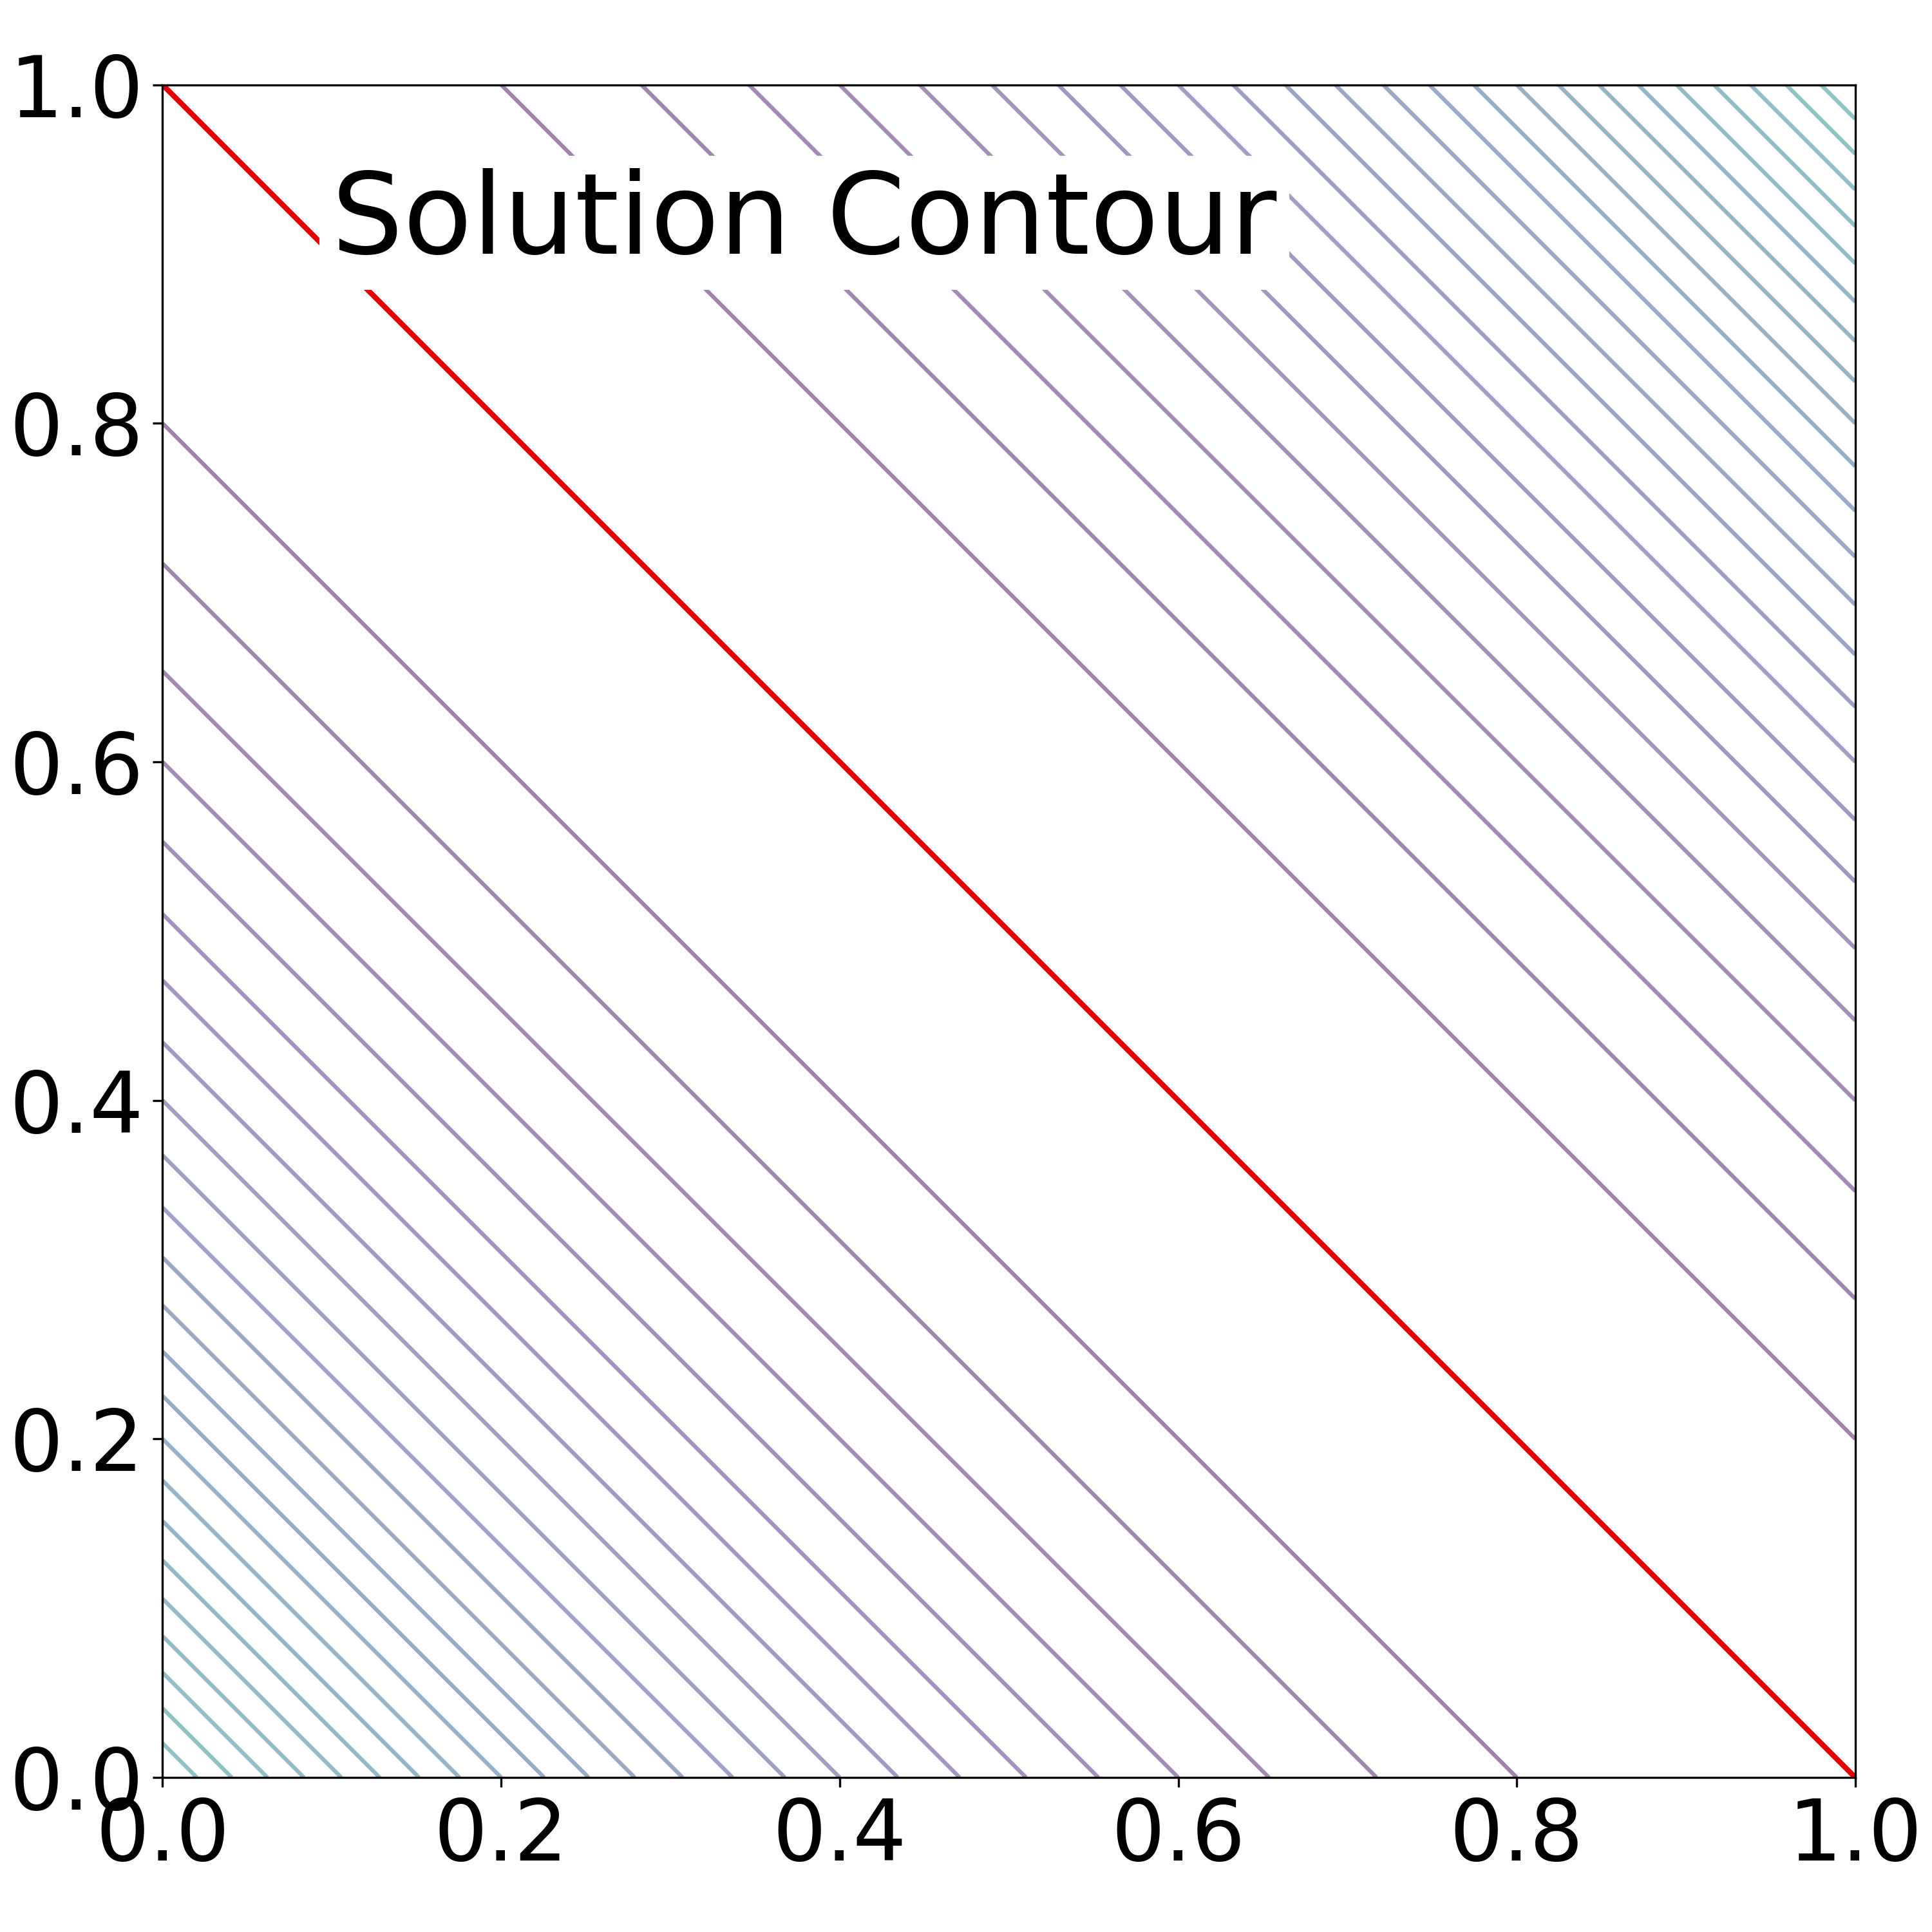
\includegraphics[width=0.25\linewidth]{figures/data_mismatch_contour.png}}
      {data mismatch}
    &
      \subf{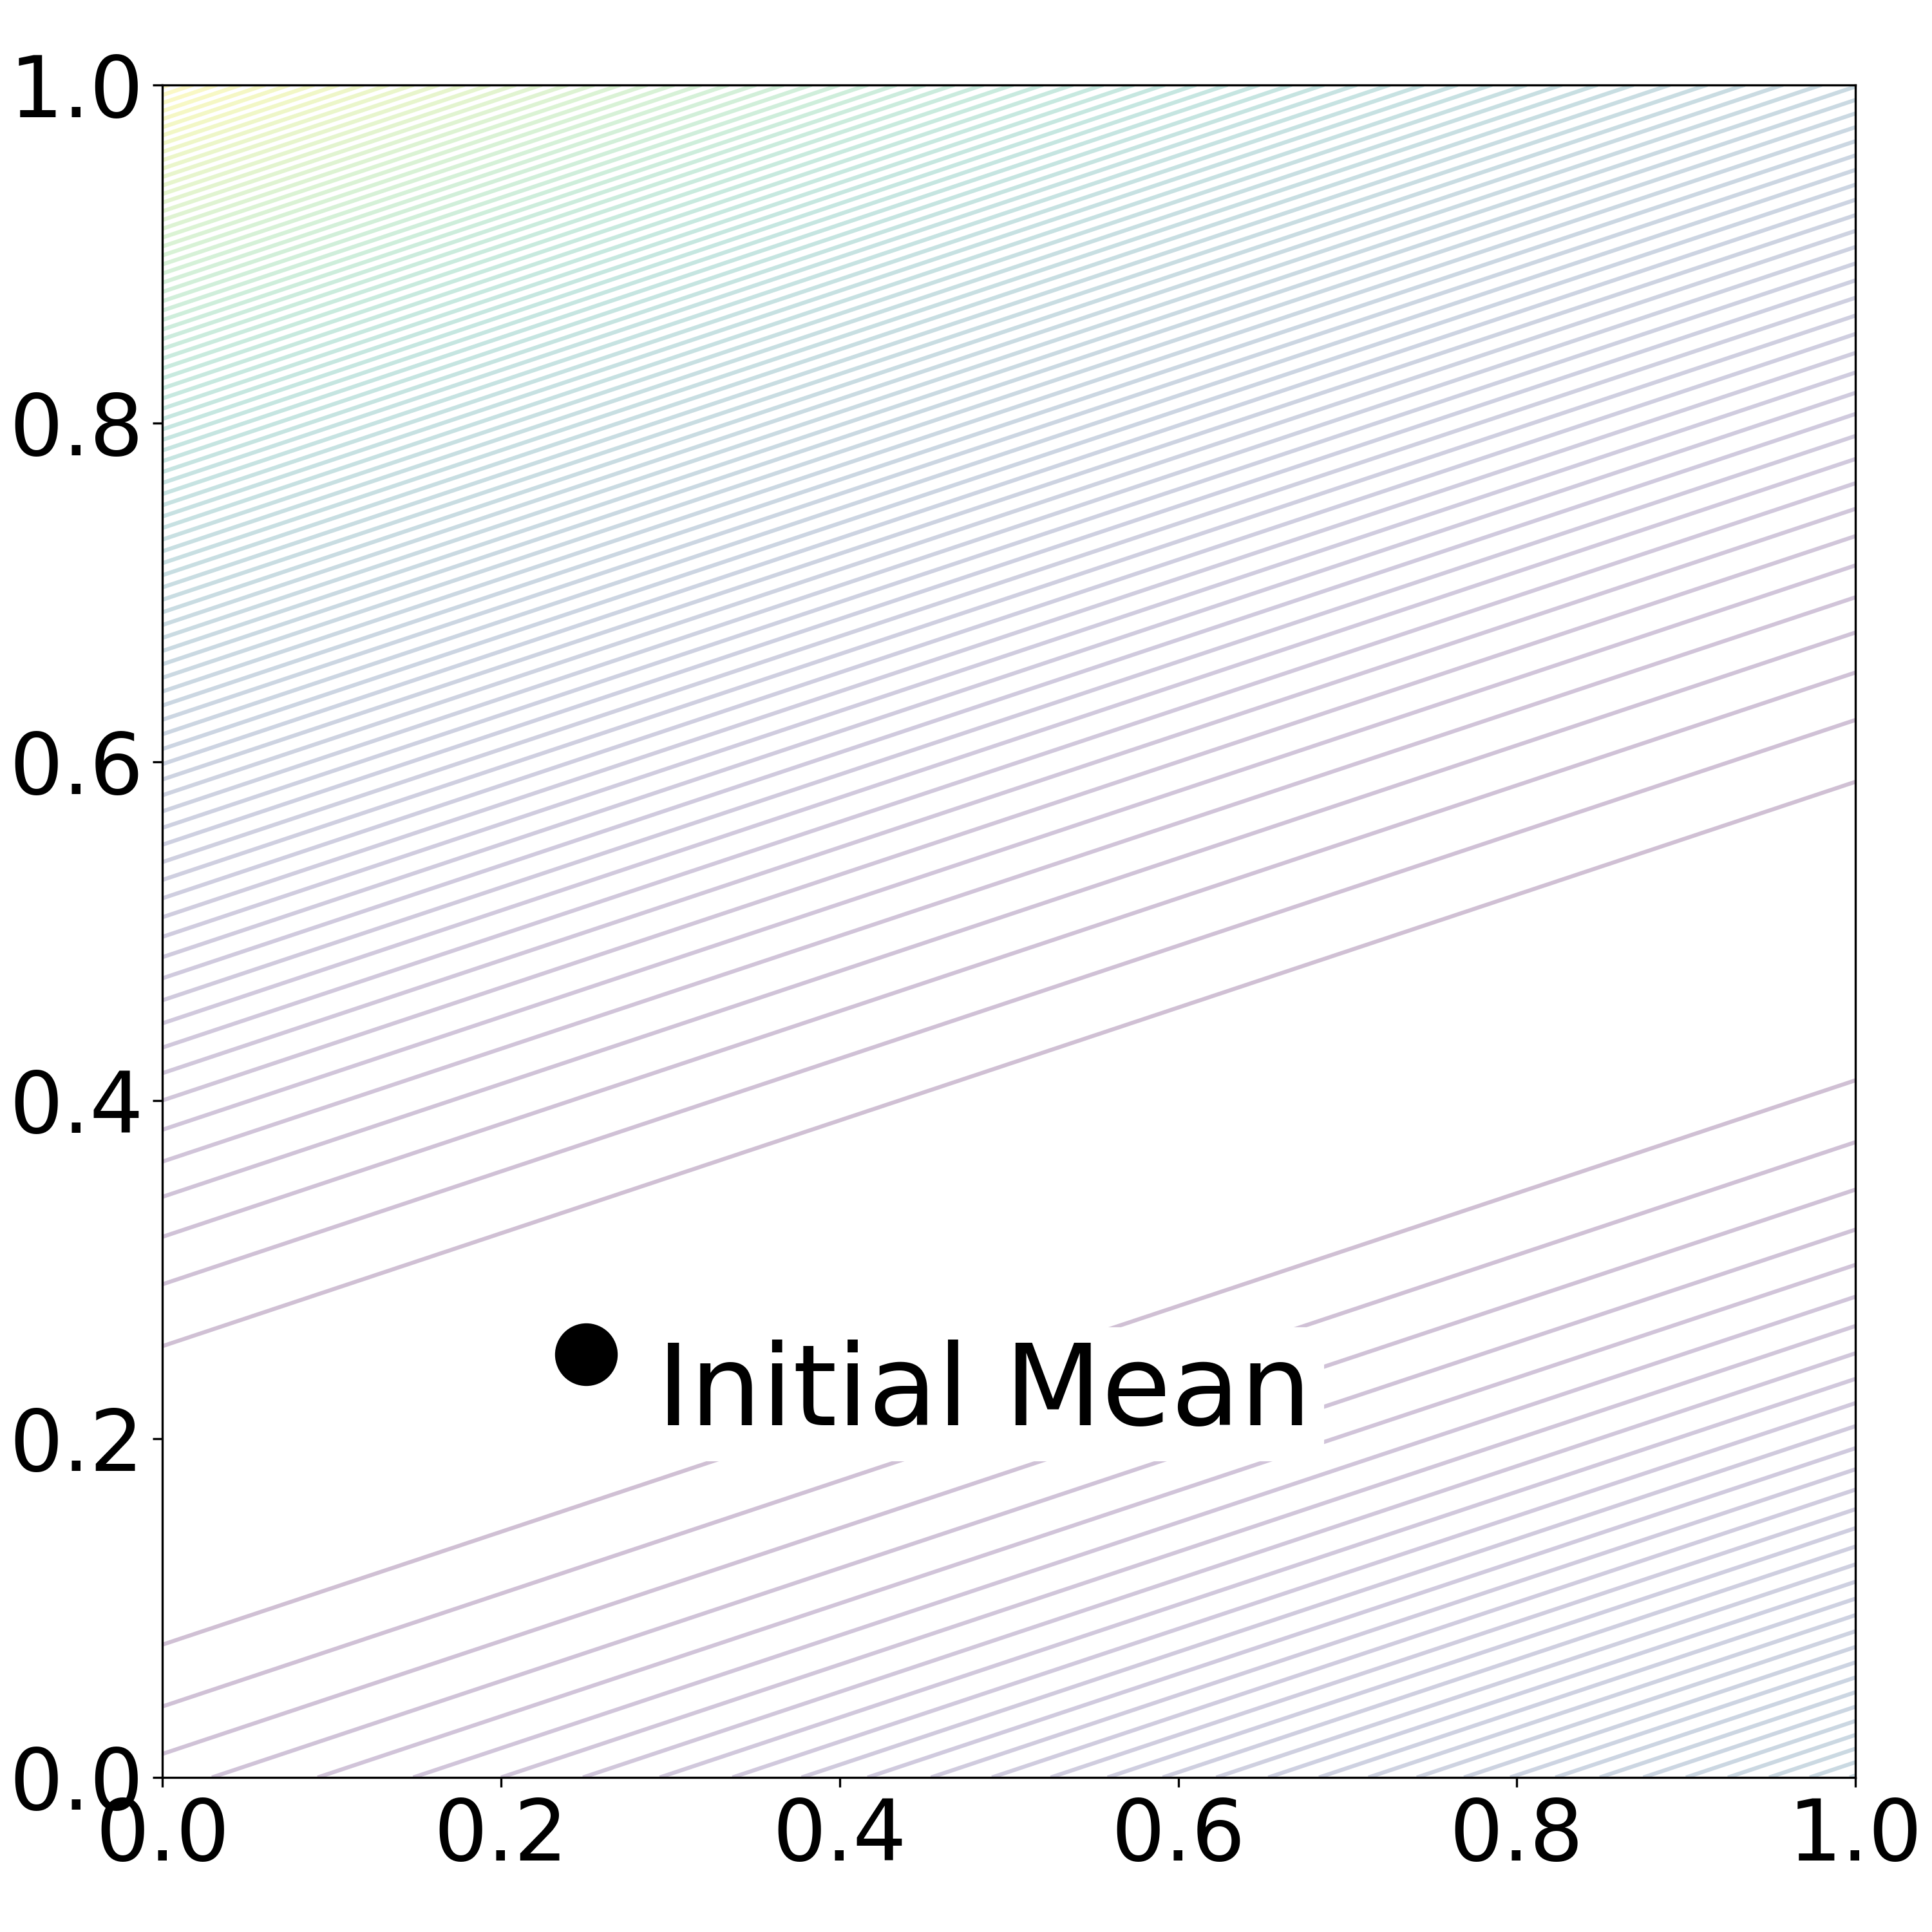
\includegraphics[width=0.25\linewidth]{figures/consistent_contour.png}}
      {modified regularization}
    &
      \subf{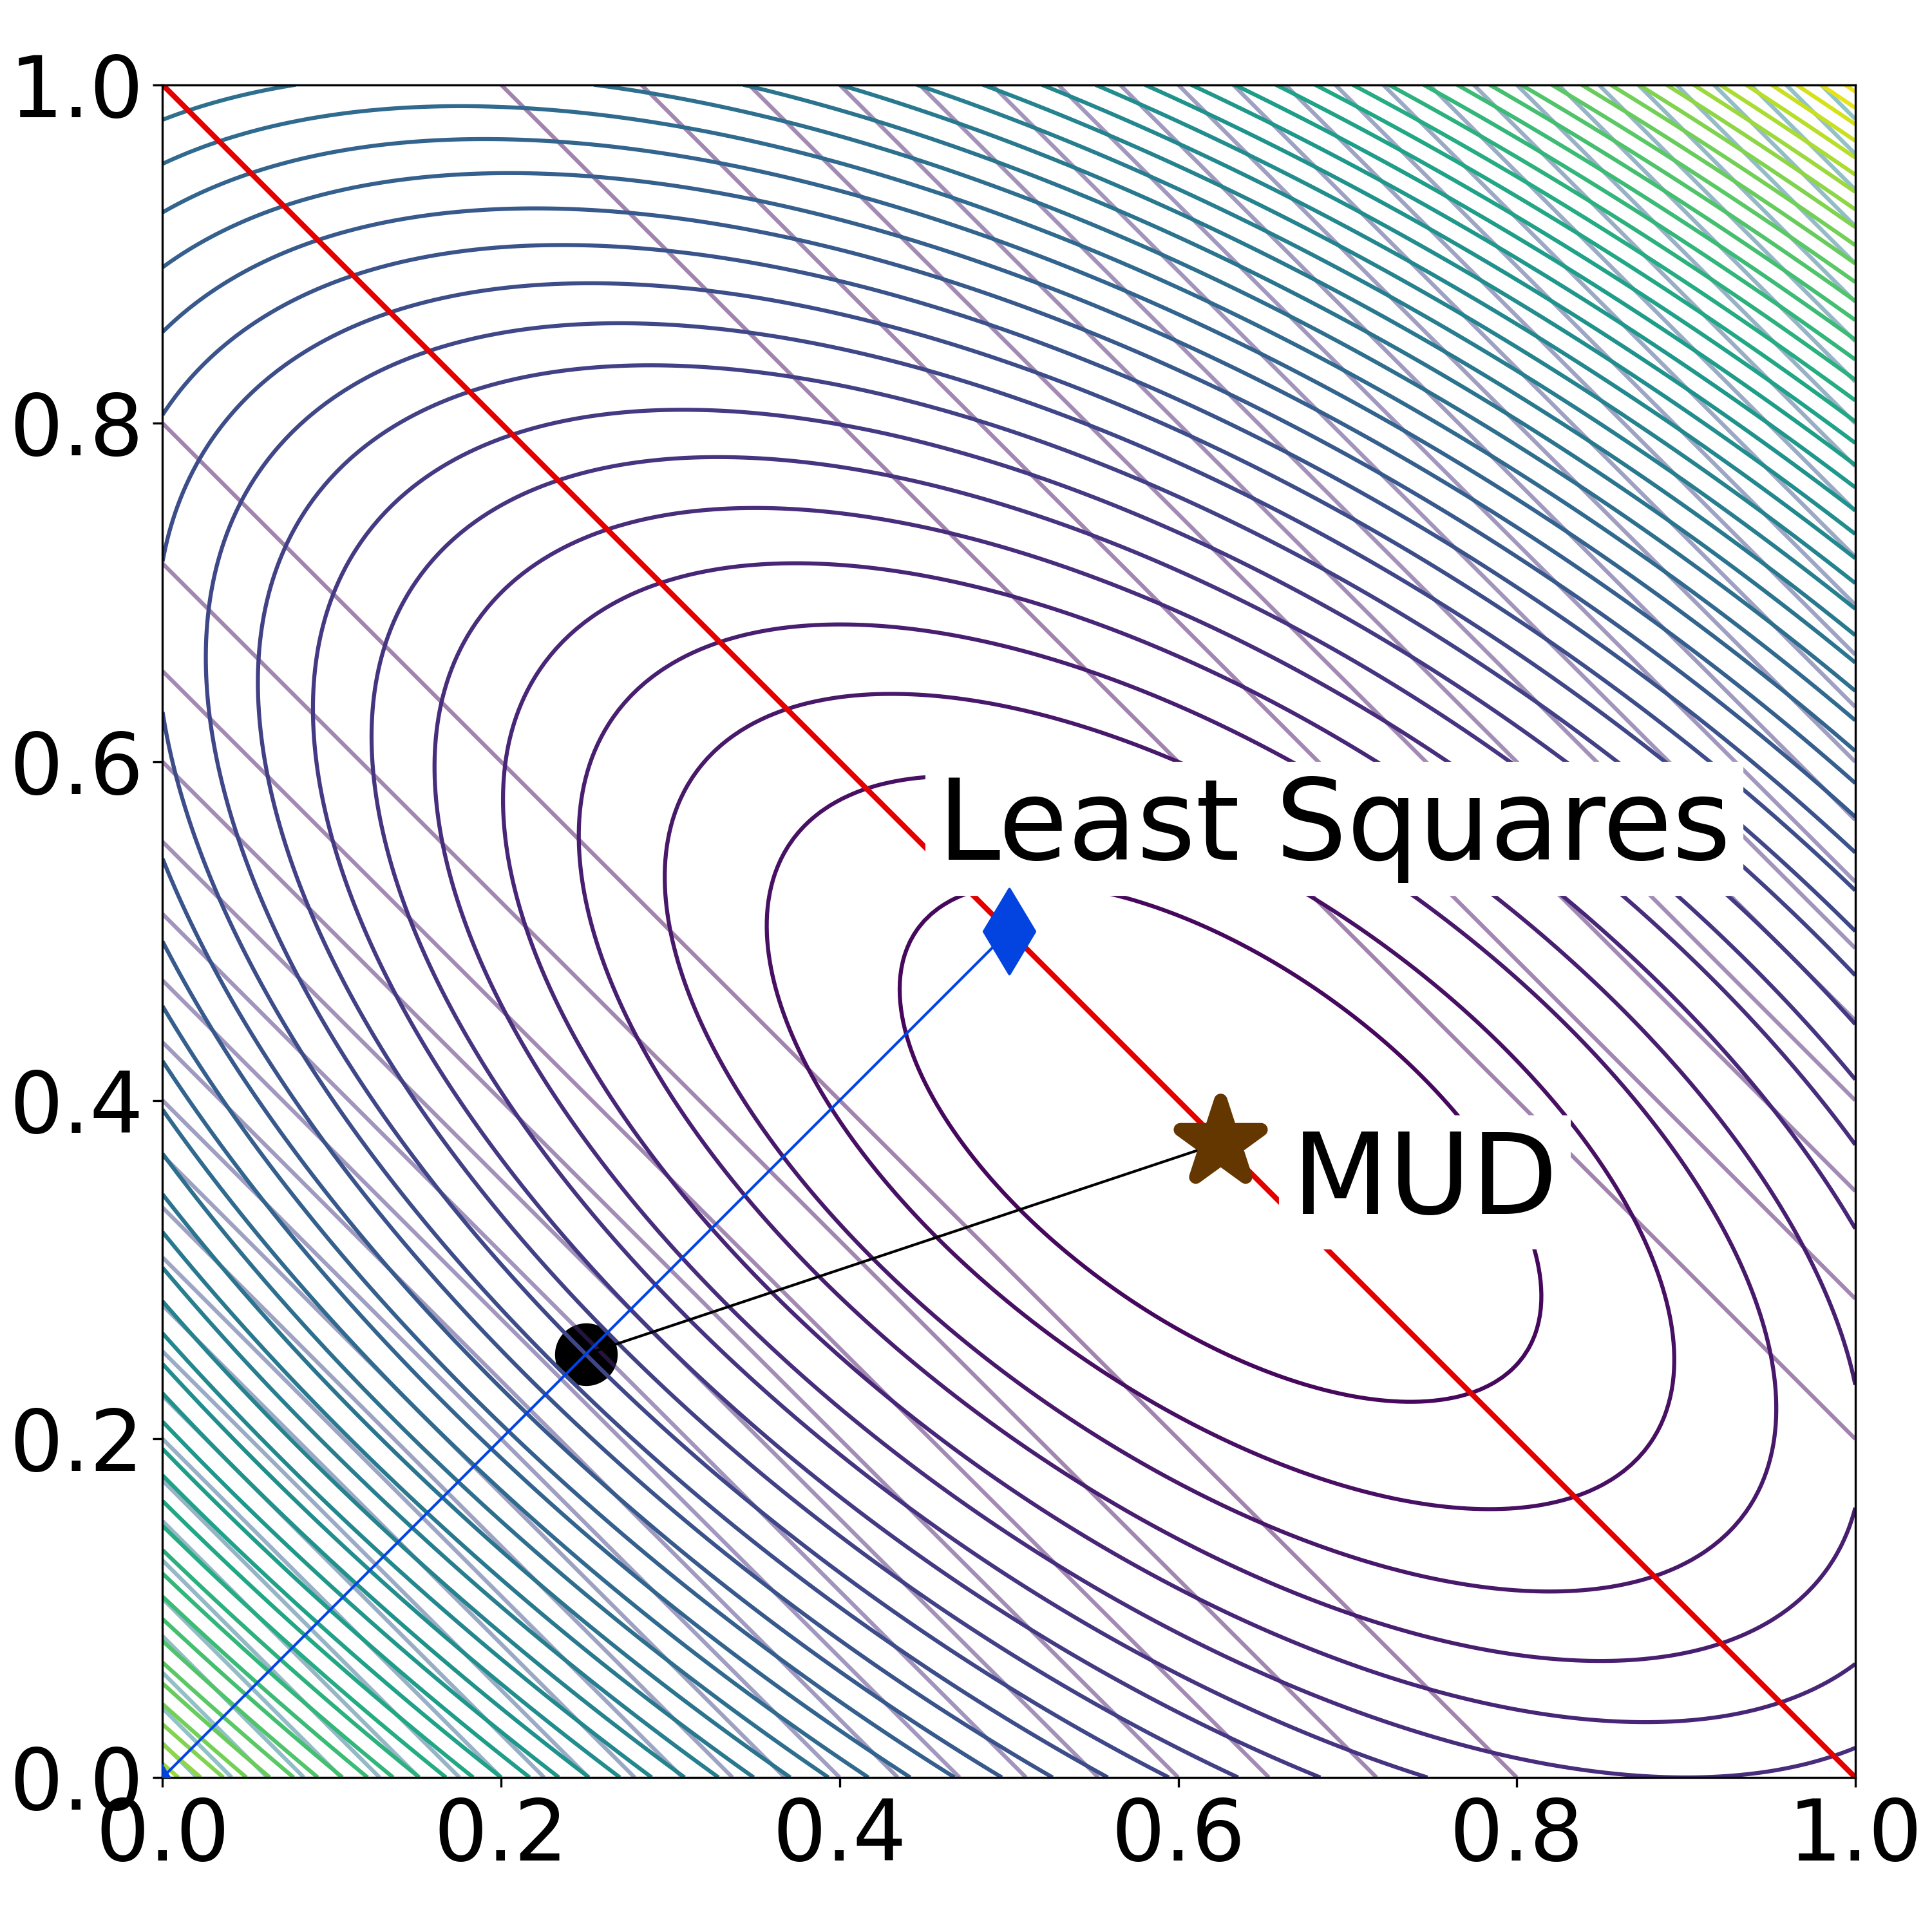
\includegraphics[width=0.25\linewidth]{figures/consistent_solution.png}}
       {updated density}
    \\
    \hline
  \end{tabular}

  \caption{Gaussian data mismatch for a 2-to-1 linear map (left plots). Gaussian initial/prior induce different regularization terms (middle plots), which leads to different optimization functions (right plots) and parameter estimates.}
  \label{fig:regularization}
\end{figure}


\end{figure}

\end{frame}


%%%%%%%%%%%%%%%%%%%%%%%%%%%%%%%%%%%%%%%%%%%%%%%%%%%%%%%%%%%
\subsection{Closed-Form Solutions}
%%%%%%%%%%%%%%%%%%%%%%%%%%%%%%%%%%%%%%%%%%%%%%%%%%%%%%%%%%%

\begin{frame}[t]
%\vskip 25pt
\centering

The posterior covariance is formally given by

\begin{equation}\label{eq:map_cov}
\Sigma_\text{post} := ( A^\top {\Sigma}_\text{obs}^{-1} A + \initialCov^{-1} )^{-1}.
\end{equation}

Applying Woodbury identity and~\eqref{eq:predictCov}, we rewrite the posterior covariance:

\begin{equation}\label{eq:map_cov_analytical}
\Sigma_\text{post} = \initialCov - \initialCov A^\top \left[\predictedCov + \observedCov\right]^{-1} A \initialCov
\end{equation}

Can now interpret $\Sigma_\text{post}$ as a rank $d$ correction (or update) of $\initialCov$. \\
$\predictedCov + \observedCov$ is invertible because it is the sum of two s.p.d matrices. \\
We rewrite the closed form expression for the MAP poing given in \cite{Tarantola_book} as

\begin{equation}\label{eq:map-point-analytical}
\param^{\text{MAP}} = \param_0 + \Sigma_\text{post} A^\top \observedCov^{-1} (\observedMean - b - A\param_0).
\end{equation}

\end{frame}


%%%%%%%%%%%%%%%%%%%%%%%%%%%%%%%%%%%%%%%%%%%%%%%%%%%%%%%%%%%
\begin{frame}[t]

We define
\begin{equation}\label{eq:eff_reg}
	R := \nolinebreak \initialCov^{-1} - \nolinebreak A^\top \predictedCov^{-1} A.
\end{equation}

Using this $R$, rewrite $J(\param)$ as

\begin{equation}\label{eq:dci-objective-alt}
J(\param):= \norm{\observedMean - Q(\param)}_{\observedCov^{-1}}^2 + \norm{\param - \param_0}_{R}^2.
\end{equation}

\vskip 12pt
In this form, we identify $R$ as the {\em effective regularization} in $J(\param)$ due to the formulation in the data-consistent framework.
\begin{equation}
	\updatedCov := \left(A^\top \observedCov^{-1} A + R\right)^{-1}.
\end{equation}

Since $R$ is not invertible, Woodbury's identity cannot be applied (yet).
\end{frame}

%%%%%%%%%%%%%%%%%%%%%%%%%%%%%%%%%%%%%%%%%%%%%%%%%%%%%%%%%%%
\begin{frame}[t]
%\vskip 25pt
\centering
We derive using several identities
\begin{equation}\label{eq:updatedCov_final}
	\updatedCov = \initialCov - \initialCov A^\top \predictedCov^{-1}\left[\predictedCov-\observedCov\right]\predictedCov^{-1}A\initialCov.
\end{equation}

\vskip 12pt
Substitute $\updatedCov$ for $\Sigma_\text{post}$ in \eqref{eq:map-point-analytical} to write the point that minimizes $J$ as:

\begin{equation}\label{eq:mud-point-analytical-alt}
\param^{\text{MUD}} = \param_0 + \updatedCov A^\top \observedCov^{-1} (\observedMean - b - A\param_0).
\end{equation}

\vskip 12pt
Substituting~\eqref{eq:updatedCov_final} into~\eqref{eq:mud-point-analytical-alt} and simplifying, we have
\begin{equation}\label{eq:mud-point-analytical-final}
	\mudpt = \param_0 + \initialCov A^\top \predictedCov^{-1}(\observedMean - b - A\param_0).
\end{equation}

\end{frame}

\begin{frame}[t]

\centering
Predictability assumption:\\
smallest predicted > largest observed (eigenvalues of covariances)

\vskip 12pt
\begin{thm}\label{thm:MUD_existence_uniqueness}
Suppose  $Q(\param)=A\param+b$ for some full rank $A\in\RR^{d\times p}$ with $d\leq p$ and $b\in\RR^d$.
If $\initial \sim N(\param_0,\initialCov)$, $\observed\sim N(\observedMean,\observedCov)$, and the predictability assumption holds, then
\begin{enumerate}[(a)]
\item There exists a unique parameter, denoted by $\mudpt$, that maximizes $\updated$.
\item $Q(\mudpt) = \observedMean$.
\item If $d=p$, $\mudpt$ is given by $A^{-1}$. If $d<p$, $\mudpt$ is given by~\eqref{eq:mud-point-analytical-final} and the covariance associated with this point is given by~\eqref{eq:updatedCov_final}.
\end{enumerate}
\end{thm}

\end{frame}

%%%%%%%%%%%%%%%%%%%%%%%%%%%%%%%%%%%%%%%%%%%%%%%%%%%%%%%%%%%
\subsection{Impact of Information Content}
%%%%%%%%%%%%%%%%%%%%%%%%%%%%%%%%%%%%%%%%%%%%%%%%%%%%%%%%%%%

\begin{frame}[t]{\it The one where we show how rank and dimension impact our solutions.}
%\vskip 25pt
\centering
\centering
Example: scaling random diagonal initial covariances

\begin{figure}[htbp]
  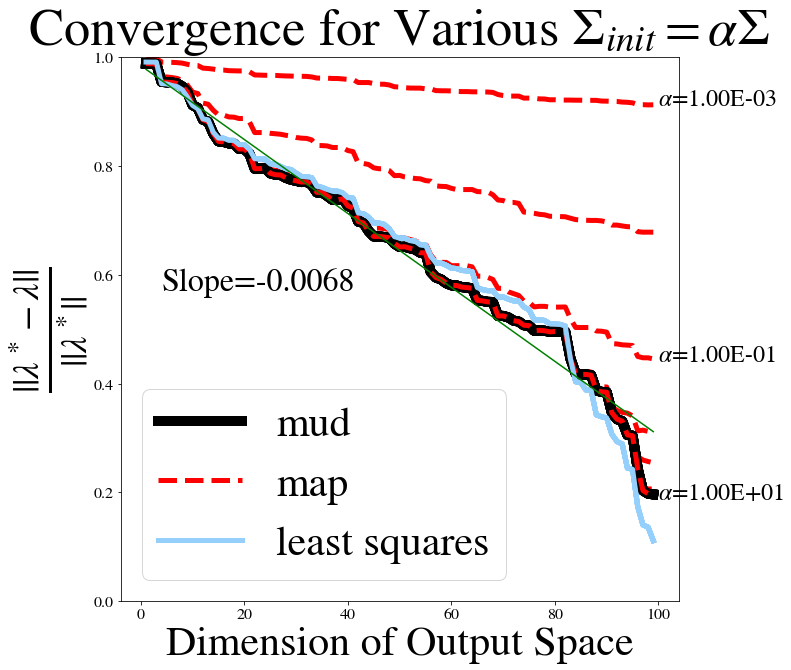
\includegraphics[width=0.475\linewidth]{figures/lin/lin-dim-cov-convergence}
  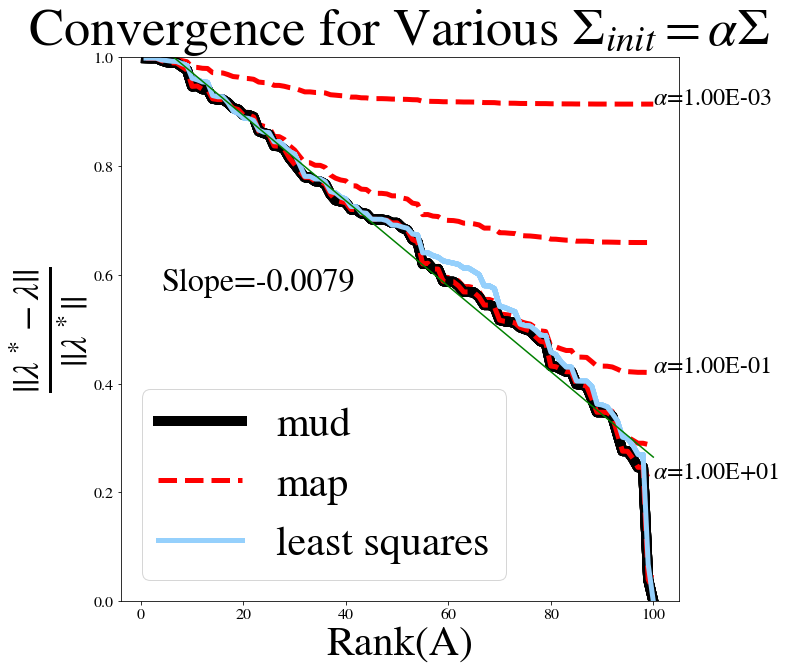
\includegraphics[width=0.475\linewidth]{figures/lin/lin-rank-cov-convergence}
\caption{
	Relative errors between $\paramref$ and (i) the least squares solution obtained through {\tt numpy}'s {\tt linalg.pinv} module, (ii) the closed-form solution for the MUD point given in Eq~\eqref{eq:mud-point-analytical-final}, and (iii) the MAP point.
  (Left): Error for increasing dimensions of $D$ for $A$ taken to be a Gaussian Random Map.
  (Right): Error for increasing row-rank of $A$, generated with Gaussian vectors and a SVD.
}
\label{fig:lin-error}
\end{figure}

\end{frame}


%%%%%%%%%%%%%%%%%%%%%%%%%%%%%%%%%%%%%%%%%%%%%%%%%%%%%%%%%%%
\subsection{Data-Driven QoI Maps}
%%%%%%%%%%%%%%%%%%%%%%%%%%%%%%%%%%%%%%%%%%%%%%%%%%%%%%%%%%%

\begin{frame}[t]{\it The one where we leverage this framework for general streams of data.}
\centering
Suppose $\exists \; d$ measurement devices generating repeated noisy data. \\
\vskip 12pt
For each $1\leq j\leq d$, denote by $\mathcal{M}_j(\paramref)$ the $j$th measurement device. \\

$N_j$ is number of noisy data obtained for $\mathcal{M}_j(\paramref)$.
\vskip 12pt
$d_{j,i}$ is the $i$th noisy datum for the $j$th measurement, where $1\leq i\leq N_j$.

\vskip 12pt
Assume an unbiased additive error model for the measurement noise,
with independent identically distributed (i.i.d.) Gaussian errors so that
\begin{equation}\label{eq:obs_data_error}
	d_{j,i} = M_j(\param^\star) + \xi_i, \ \xi_i\sim N(0,\sigma_j^2), \ \ 1\leq i\leq N_j.
\end{equation}

\vskip 12pt
We now construct a $d$-dimensional vector-valued map from data obtained on the $d$ measurement devices.

\end{frame}


%%%%%%%%%%%%%%%%%%%%%%%%%%%%%%%%%%%%%%%%%%%%%%%%%%%%%%%%%%%
\begin{frame}[t]{\it The one with the Weighted Mean Error (WME) map.}
\centering

The weighted mean error (WME) map, denoted by $Q_\text{WME}(\param)$ has $j$th component, denoted by $Q_{\text{WME},j}(\param)$, given by

\begin{equation}\label{eq:qoi_WME}
	Q_{\text{WME},j}(\param) := \frac{1}{\sqrt{N_j}} \sum_{i=1}^{N_j} \frac{M_j(\param)-d_{j,i}}{\sigma_j}.
\end{equation}

\vskip 12pt
$Q_{\text{WME},j}(\paramref)$ is the sample avg of $N_j$ random draws from an i.i.d.~$N(0,N_j)$.\\
By assumption, the observed data are generated according to the fixed true physical parameter vector given by $\paramref$ in \eqref{eq:obs_data_error}.

\vskip 12pt
Subsequently, each component of $Q_\text{WME}(\paramref)$ is a random draw from an $N(0,1)$ distribution.\\
Therefore, with this choice of data-defined QoI map, we specify $\observed$ as a $N(\mathbf{0}_{d\times 1},\mathbf{I}_{d\times d})$ distribution.

\end{frame}


\begin{frame}[t]{\it The one where measurements impact the predictability assumption.}
\centering
The $j$th diagonal component of the predicted covariance matrix is given by the predicted variance associated with using the scalar-valued $Q_{\text{WME},j}$.

Then, the associated predicted variance is given by
\begin{equation}
	\frac{N_j}{\sigma_j^2} M_j\initialCov M_j^\top
\end{equation}

Since $\initialCov$ is assumed to be non-degenerative and $M_j$ is a non-trivial row vector, this predicted variance grows linearly with $N_j$.\\
\vskip 12pt
In other words, the $j$th diagonal component of the predicted covariance has the form $\beta_j N_j$ for some $\beta_j>0$.
\end{frame}


\begin{frame}[t]
\centering
Let $N_{\text{min},j}$ denote the minimum $N_j$ for $1\leq j\leq N$ necessary to make the $j$th diagonal components sufficiently large so that the smallest eigenvalue of the predicted covariance is larger than $1$.

\vskip 12pt
The following result is now an immediate consequence of Theorem~\ref{thm:MUD_existence_uniqueness}:\\

\begin{corollary}\label{cor:MUD_wme}
If $\initial \sim N(\param_0,\initialCov)$ and data are obtained for $d$ linearly independent measurements on $\pspace$ with an additive noise model with i.i.d. Gaussian noise for each measurement, then {\bf there exists a minimum number of data points obtained for each of the measurements} such that there exists a unique $\mudpt$ and $Q_\text{WME}(\mudpt) = 0$.
\end{corollary}


\end{frame}

%%%%%%%%%%%%%%%%%%%%%%%%%%%%%%%%%%%%%%%%%%%%%%%%%%%%%%%%%%%
\subsection{Nonlinear Examples}
%%%%%%%%%%%%%%%%%%%%%%%%%%%%%%%%%%%%%%%%%%%%%%%%%%%%%%%%%%%


%%%%%%%%%%%%%%%%%%%%%%%%%%%%%%%%%%%%%%%%%%%%%%%%%%%%%%%%%%%
\begin{frame}[t]{\it The one where we violate some assumptions.}
%\vskip 25pt
\centering
Consider the exponential decay problem with uncertain decay rate $\param$:
$$
\begin{cases}
\frac{\partial u}{\partial t} & = \param u(t), \ 0<t\leq 3, \\ u(0) &= 0.75,
\end{cases}
$$
with solution
\begin{equation}
u(t;\param) = u_0\exp(-\param t), \; u_0 = 0.75 ,
\end{equation}
and measurements begin at $t=1$.
\end{frame}


%%%%%%%%%%%%%%%%%%%%%%%%%%%%%%%%%%%%%%%%%%%%%%%%%%%%%%%%%%%
\begin{frame}[t]
\only<1>{
\begin{figure}[htb]
  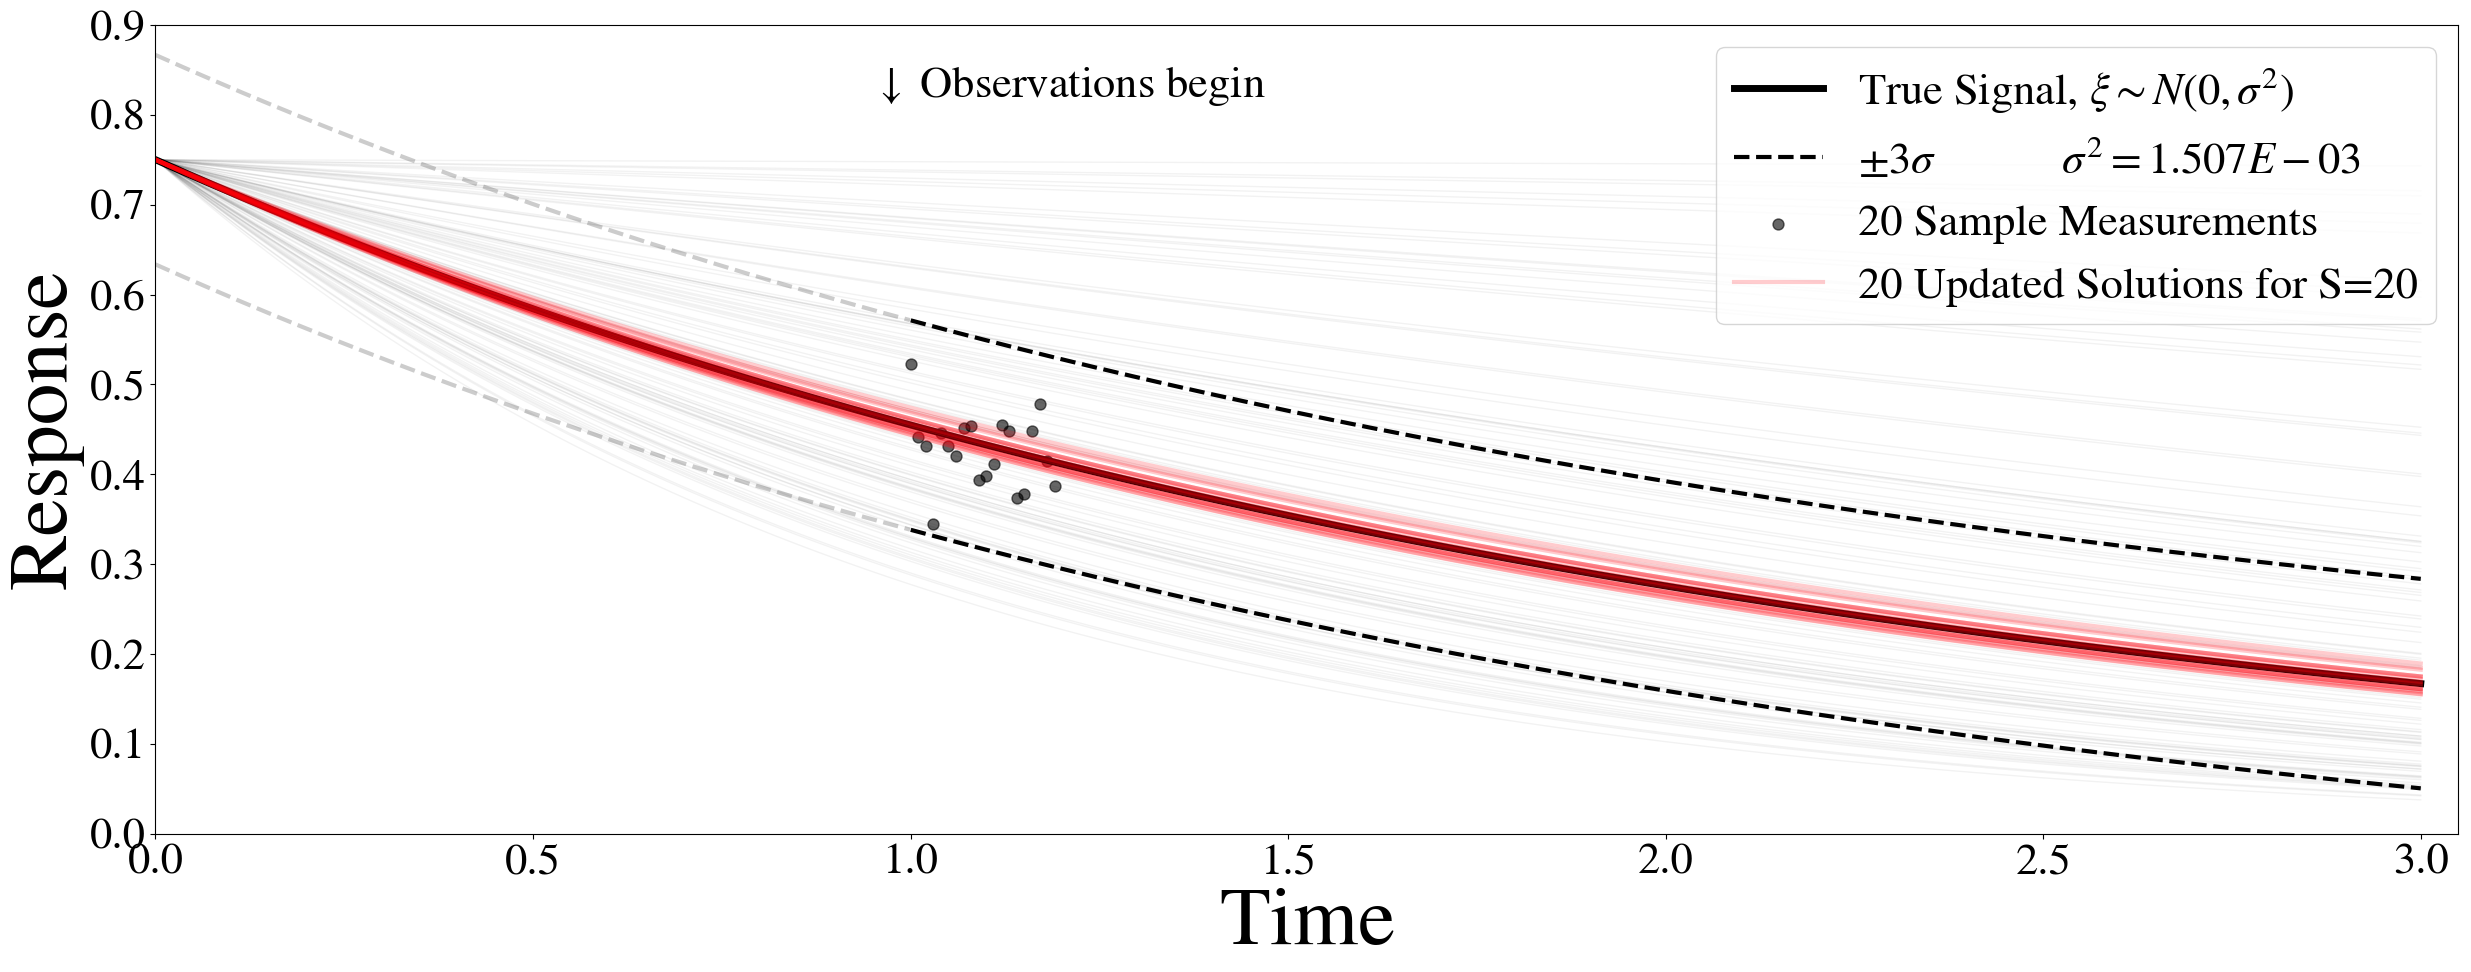
\includegraphics[width=0.8\linewidth]{figures/ode/ode_20_reference_solution.png}
  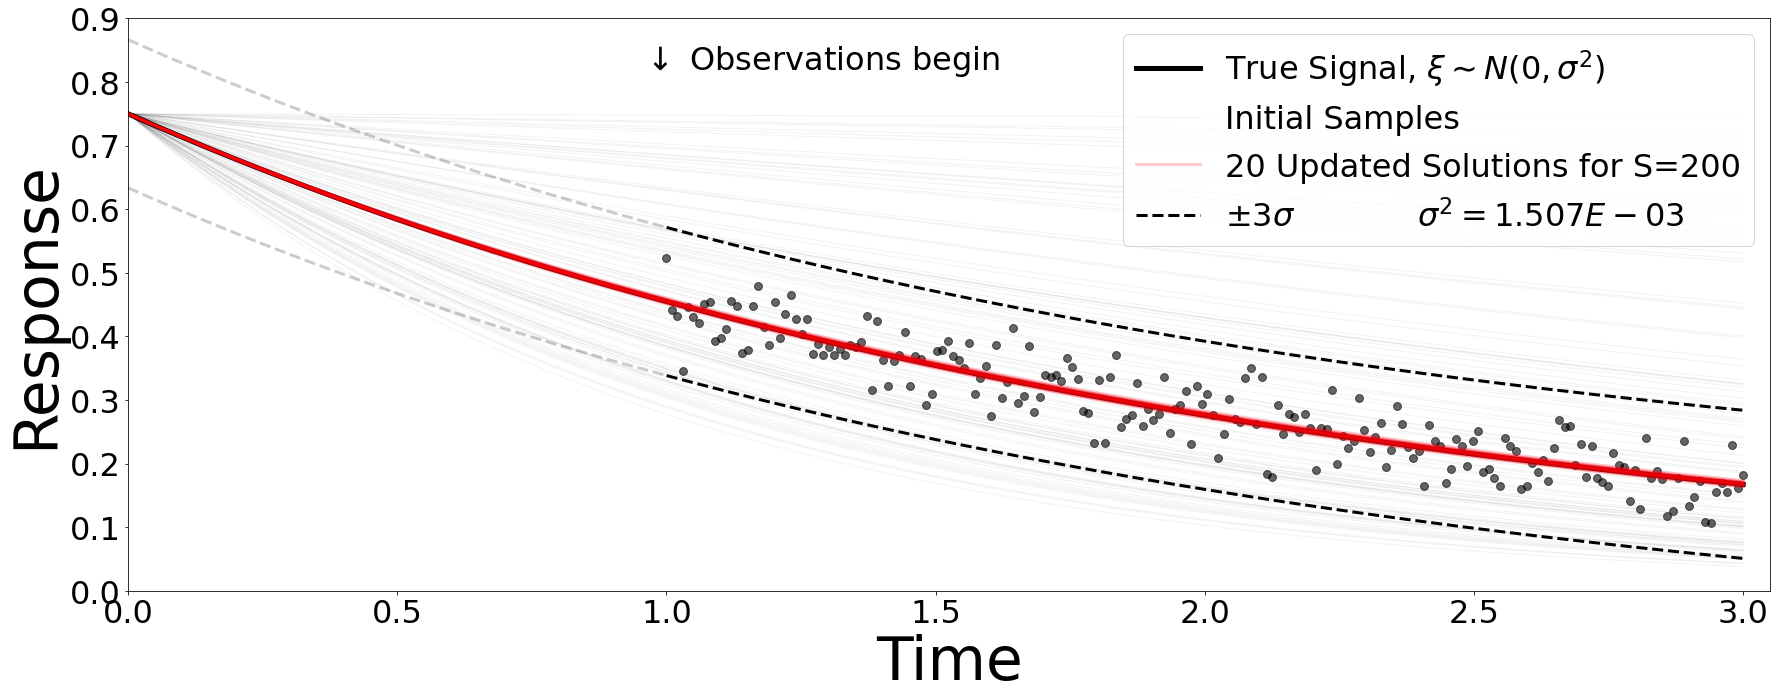
\includegraphics[width=0.8\linewidth]{figures/ode/ode_200_reference_solution.png}
  \caption{Curves for exponential decay model with various decay coefficients. Dashed curves denote 99\% probability intervals for noise. The true signal is shown in solid black.
 Curves associated with the MUD estimates for the decay coefficient computed from 20 trials are shown in light red.
 Both sets of these curves encompass the true signal for $N=20$ (top plot) and $N=200$ (bottom plot) data points.
 The light red curves are almost indistinguishable in the bottom plot as they all lie nearly on the true signal which demonstrates the overall reduction in variance in MUD estimates around the true signal when using $N=200$ data points.
  }
  \label{fig:ode-reference}
\end{figure}
}

\only<2>{
\begin{figure}[htb]
  \centering
  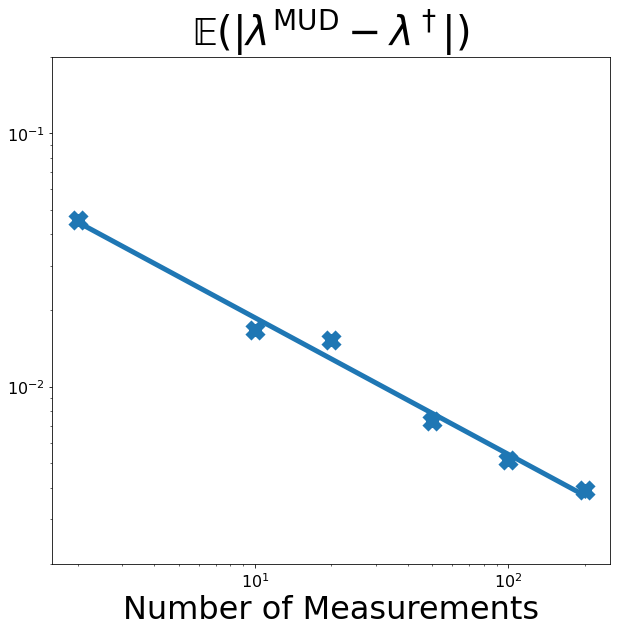
\includegraphics[width=0.45\linewidth]{figures/ode/ode_convergence_mud_obs_mean.png}
  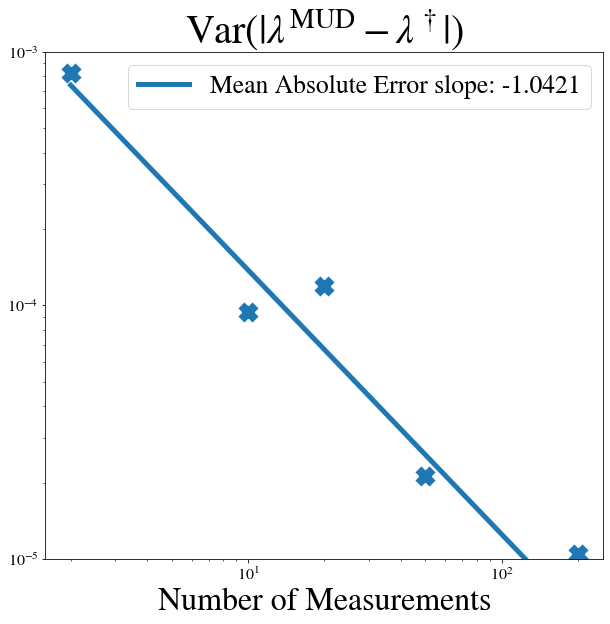
\includegraphics[width=0.45\linewidth]{figures/ode/ode_convergence_mud_obs_var.png}
  \caption{The mean (left) and variance (right) of absolute errors in MUD estimates as a function of the number of data points used. These statistics are computed over 20 trials.
  }
  \label{fig:ode-convergence}
\end{figure}
}

\end{frame}


%%%%%%%%%%%%%%%%%%%%%%%%%%%%%%%%%%%%%%%%%%%%%%%%%%%%%%%%%%%
\begin{frame}[t]{\it The one where we violate some assumptions.}

Consider the Poisson problem:
\begin{equation}\label{eq:pde-equation}
\begin{cases}
\hfill -\nabla \cdot \nabla u &= f(x), \quad\text{on } x\in \Omega, \\
\hfill u &= 0, \quad\text{ on } \Gamma_T \cup \Gamma_B, \\
\hfill \frac{\partial u}{\partial \mathbf{n}} &= g(x_2), \quad\text{ on } \Gamma_L, \\
\hfill \frac{\partial u}{\partial \mathbf{n}} &= 0, \quad\text{ on } \Gamma_R,
\end{cases}
\end{equation}
where $x=(x_1, x_2) \in \Omega = (0,1)^2$ is the spatial domain.

\begin{itemize}
\item $\Gamma_T$, $\Gamma_B$, $\Gamma_L$, and $\Gamma_R$, denote the top, bottom, left, and right boundaries of this domain
\item $\frac{\partial u}{\partial \mathbf{n}}$ denotes the usual outward normal derivative.
\item The forcing function $f$ is taken to be $10\exp\left ( \norm{x - 0.5}^2 / 0.02 \right )$.
\end{itemize}

\end{frame}


%%%%%%%%%%%%%%%%%%%%%%%%%%%%%%%%%%%%%%%%%%%%%%%%%%%%%%%%%%%
\begin{frame}[t]

\begin{itemize}
\item $g(x_2)$ is unknown, and the goal is to use noisy data to estimate this unknown boundary data.
\item In other words, the parameter $\param$ now represents an uncertain function.
\item To generate the noisy data, we use $g(x_2)\propto x_2^2(x_2-1)^5$
\item Constant of proportionality chosen so $\min{g}=-3$ at $x_2=\frac{2}{7}$.
\item Piecewise-linear finite elements on a triangulation of a $36\times36$ mesh.
\item 100 randomly placed sensors in the subdomain $(0.05, 0.95)^2 \subset \Omega$.
\item Repeated $20$ times to study the subsequent variation in MUD points due to different realizations of noisy data.
\end{itemize}

\end{frame}


%%%%%%%%%%%%%%%%%%%%%%%%%%%%%%%%%%%%%%%%%%%%%%%%%%%%%%%%%%%
\begin{frame}[t]
\begin{figure}[htbp]
\centering
    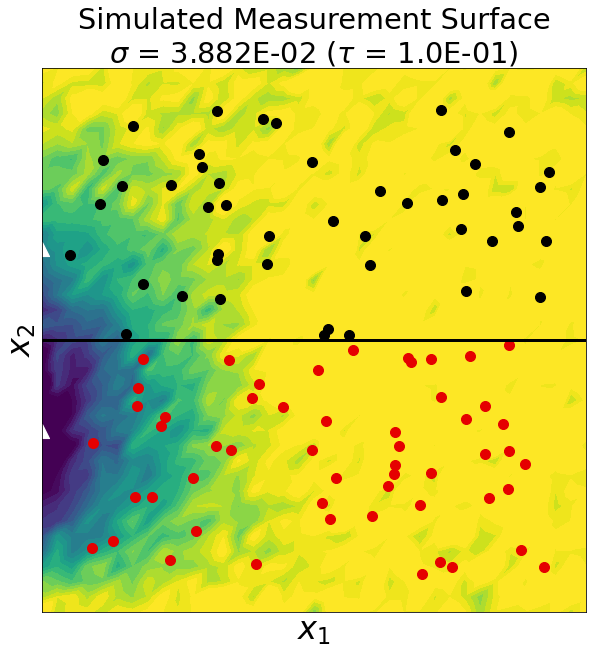
\includegraphics[width=0.5\linewidth]{figures/pde-highd/pde-highd_sensors_D2.png}
\caption{
A representative noisy perturbation of the reference response surface. Locations of the randomly chosen spatial data used to construct both $Q_{1D}$ and $Q_{2D}$ are shown as black and red dots.
}
\label{fig:pde-Q}
\end{figure}
\end{frame}


%%%%%%%%%%%%%%%%%%%%%%%%%%%%%%%%%%%%%%%%%%%%%%%%%%%%%%%%%%%
\begin{frame}[t]
\begin{figure}[htbp]
\centering
    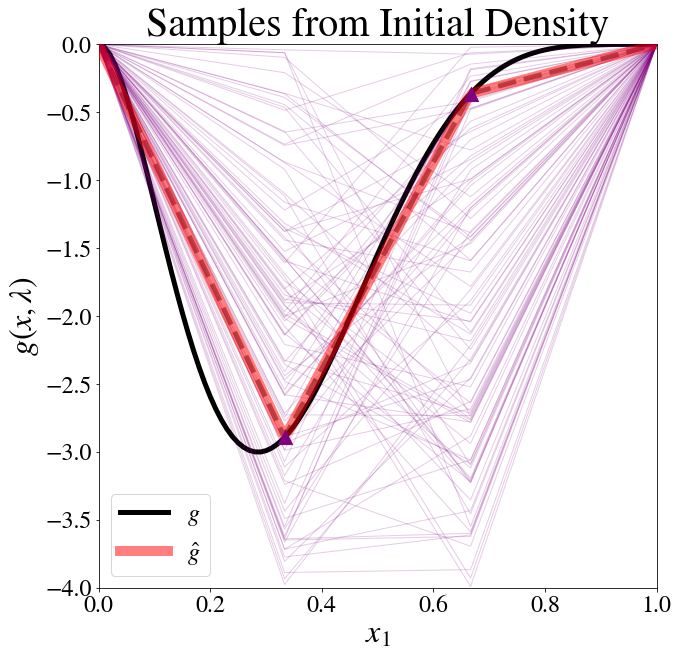
\includegraphics[width=0.325\linewidth]{figures/pde-highd/pde-highd_init_D2.png}
    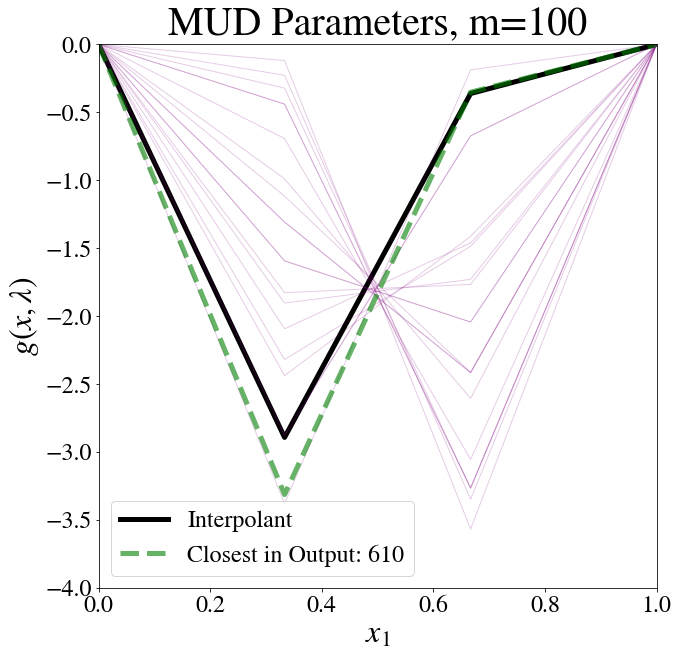
\includegraphics[width=0.325\linewidth]{figures/pde-highd/pde-highd_pair_D2-1_m100.png}
    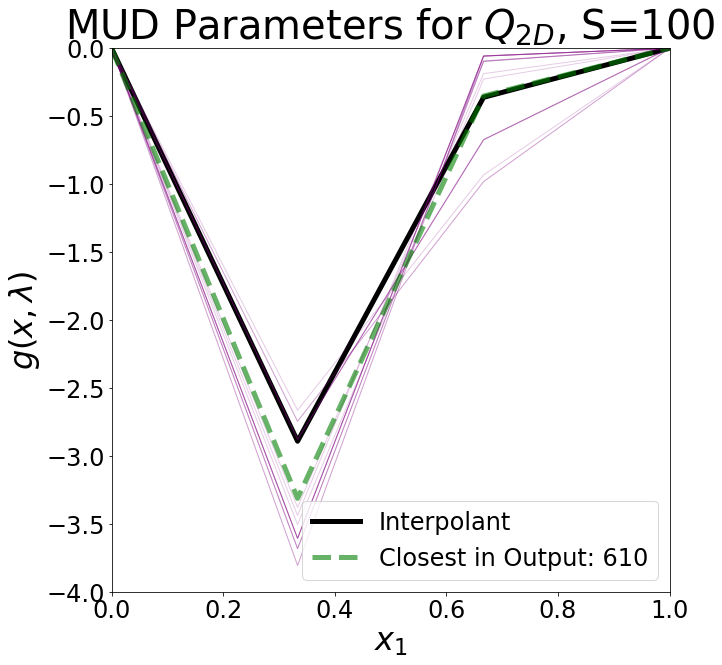
\includegraphics[width=0.325\linewidth]{figures/pde-highd/pde-highd_pair_D2-2_m100.png}
\caption{
In the left plot, the reference $g(x_2)$ is shown as the solid black curve with its interpolant onto the spline basis shown as a dotted red curve.
The dashed blue line represents the sample from parameter space which most closely predicts noiseless data, which we refer to as the projection of $g$.
The purple curves in the center and right plots show the variability in MUD estimates of $g(x_2)$ for the 20 different realizations of noisy data.
The center plot uses $Q_{1D}$ and the right plot uses $Q_{2D}$ to construct the MUD estimates.
}
\label{fig:pde-MUD}
\end{figure}
\end{frame}
